\documentclass[10pt,a4paper,twoside,openright]{book}
\usepackage[top=0.9in,bottom=0.9in,inner=1.3in,outer=0.9in]{geometry}
\usepackage{fontspec}
\setmainfont{Times New Roman}
\usepackage{setspace}
\singlespacing
\usepackage{graphicx}
\usepackage{rotating}
\usepackage{caption}
\captionsetup{font=small,labelsep=period}
\usepackage{seqsplit}
\emergencystretch=2.5em
\setcounter{tocdepth}{0}
\setcounter{secnumdepth}{0}
\begin{document}


\chapter{Development Methodology and Project Timeline}

\begin{sidewaysfigure}[p]
\centering
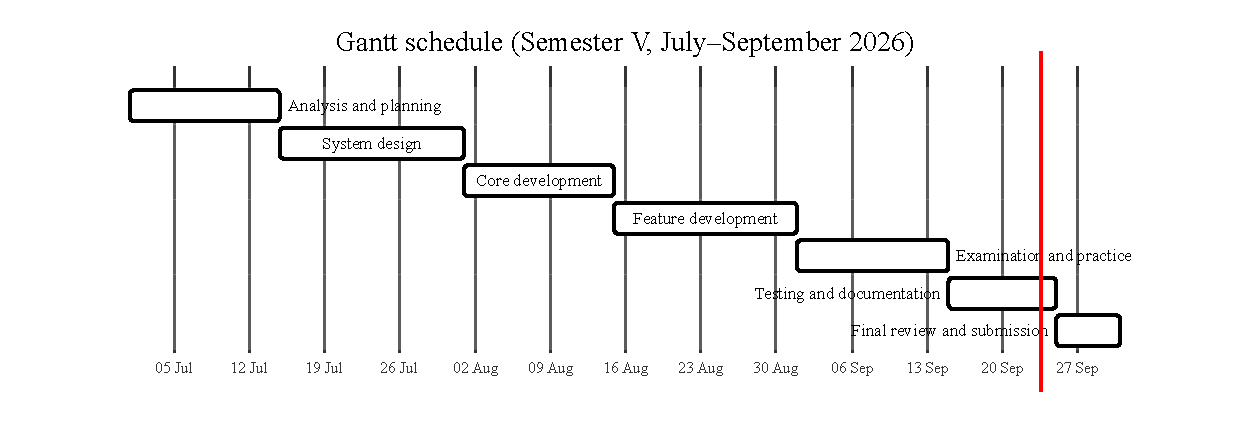
\includegraphics[width=711.5pt]{figures/gantt-chart.pdf}
\caption{Gantt chart of the seven project phases (July--September 2026).}

\end{sidewaysfigure}

\chapter{System Architecture}

\begin{sidewaysfigure}[p]
\centering
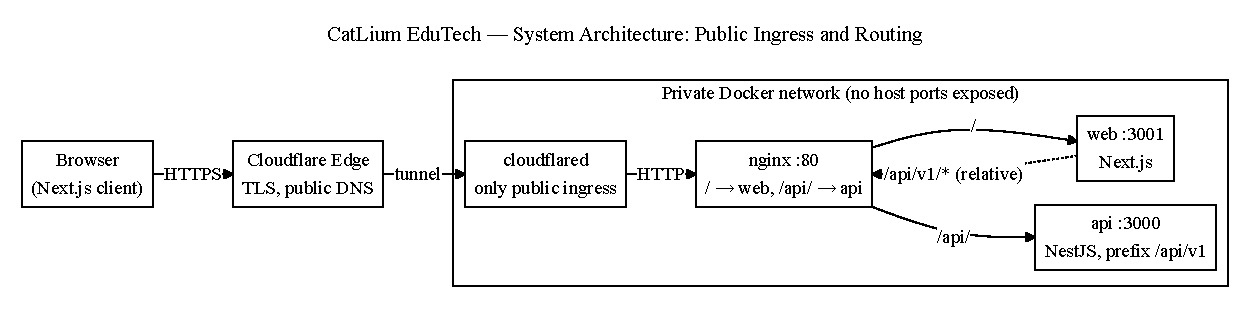
\includegraphics[width=711.5pt]{figures/system-architecture-ingress-bw.pdf}
\par\vspace{1.5ex}
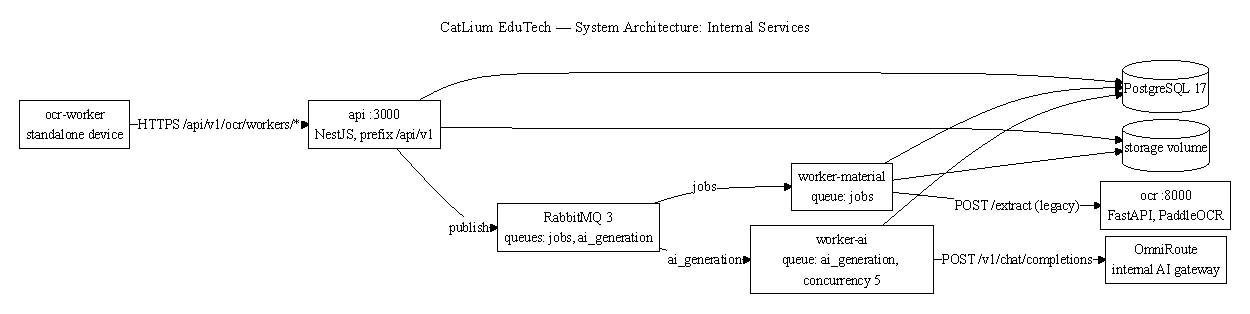
\includegraphics[width=711.5pt]{figures/system-architecture-services-bw.pdf}
\caption{System architecture and deployment topology: (left) the single public
ingress through the Cloudflare Tunnel and the internal nginx routing; (right)
the internal services on the private Docker network and their data flows.}

\end{sidewaysfigure}
\begin{sidewaysfigure}[p]
\centering
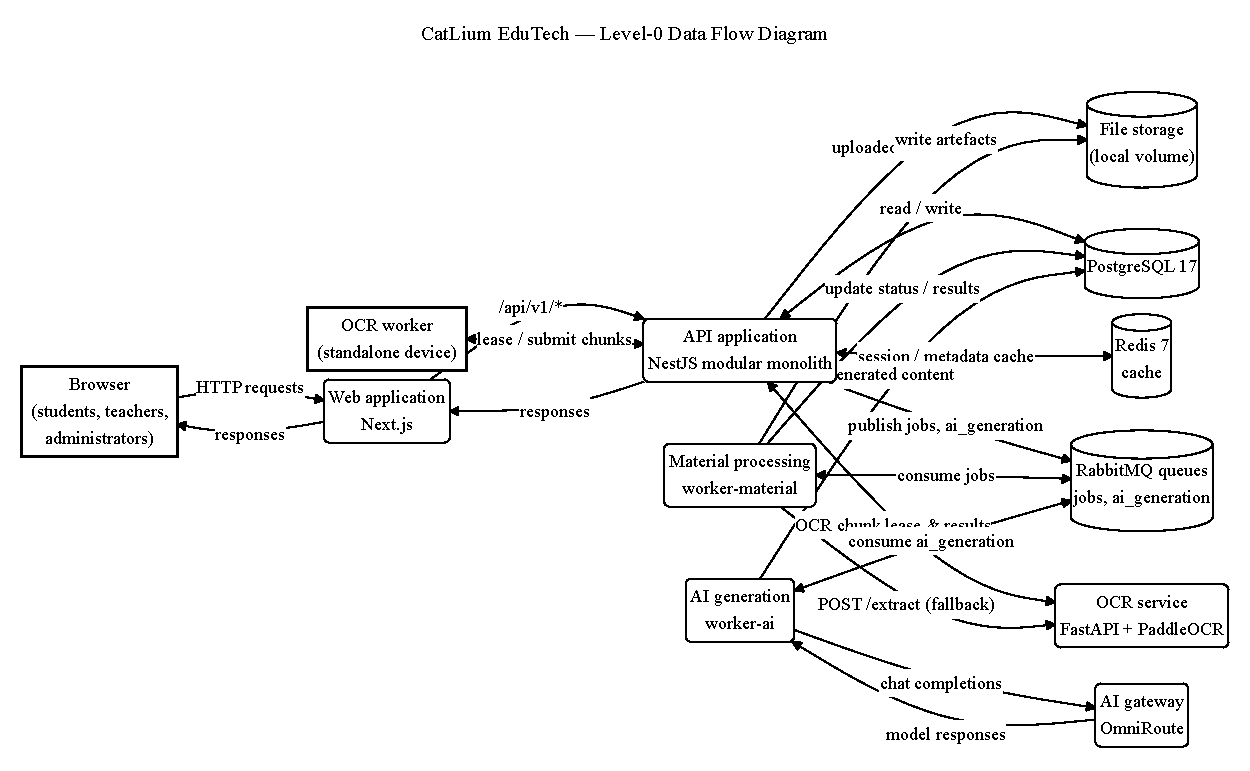
\includegraphics[width=649pt]{figures/dfd-bw.pdf}
\caption{Level-0 data flow diagram of the system.}

\end{sidewaysfigure}
\begin{sidewaysfigure}[p]
\centering
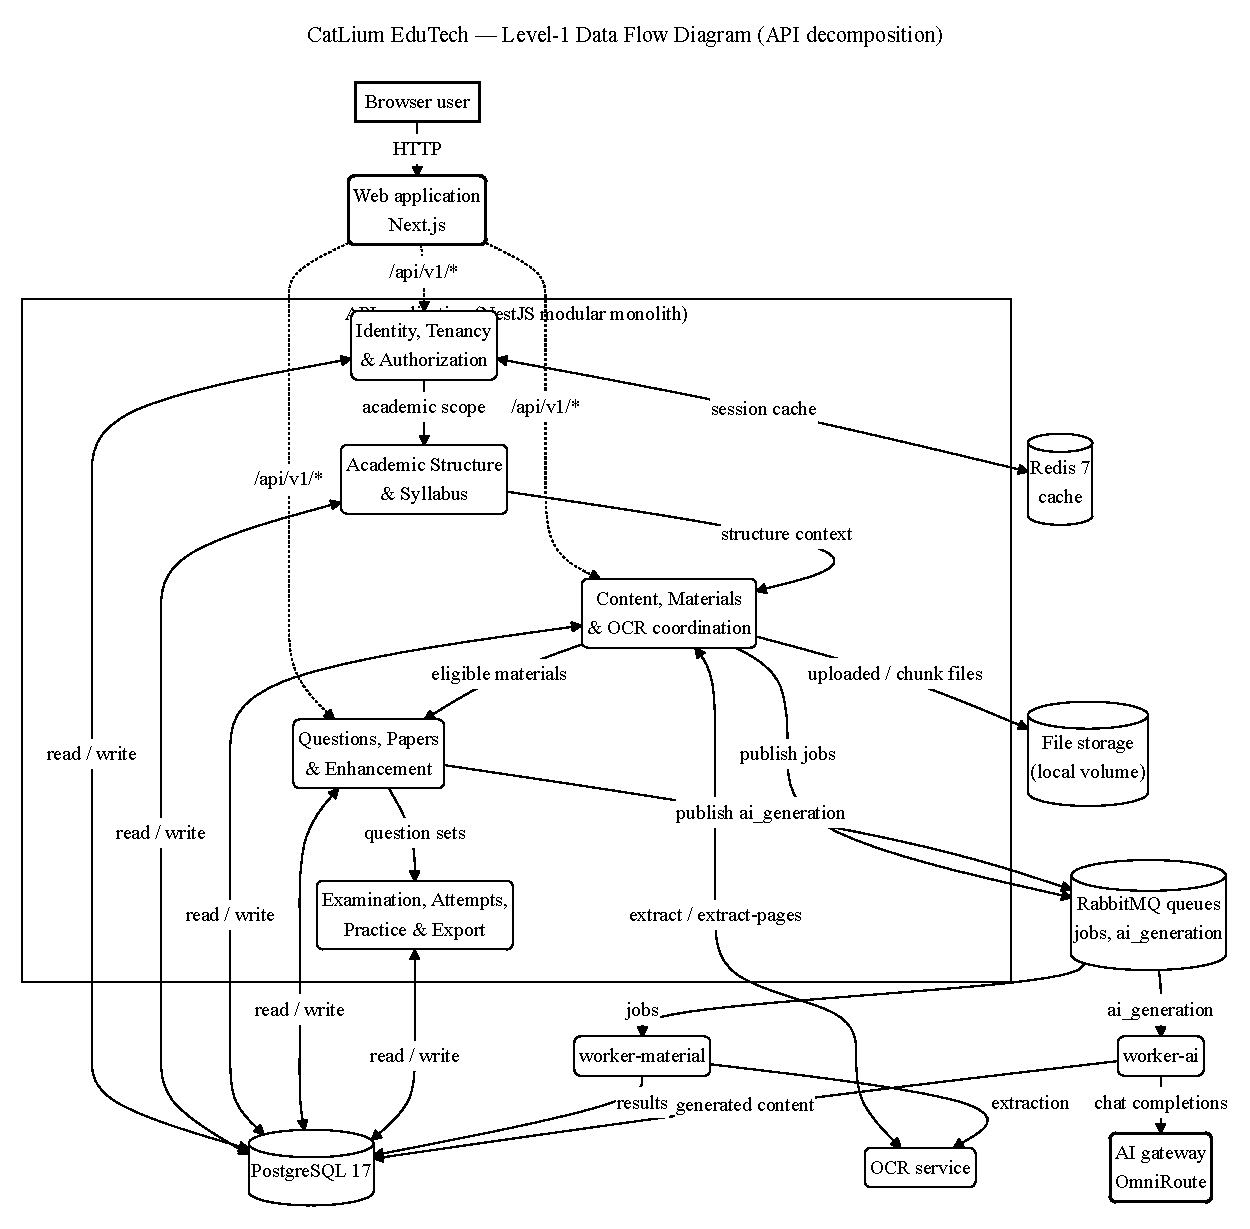
\includegraphics[width=407pt]{figures/dfd-level1-bw.pdf}
\caption{Level-1 data flow diagram: decomposition of the API application into
its principal functional areas.}

\end{sidewaysfigure}
\begin{sidewaysfigure}[p]
\centering
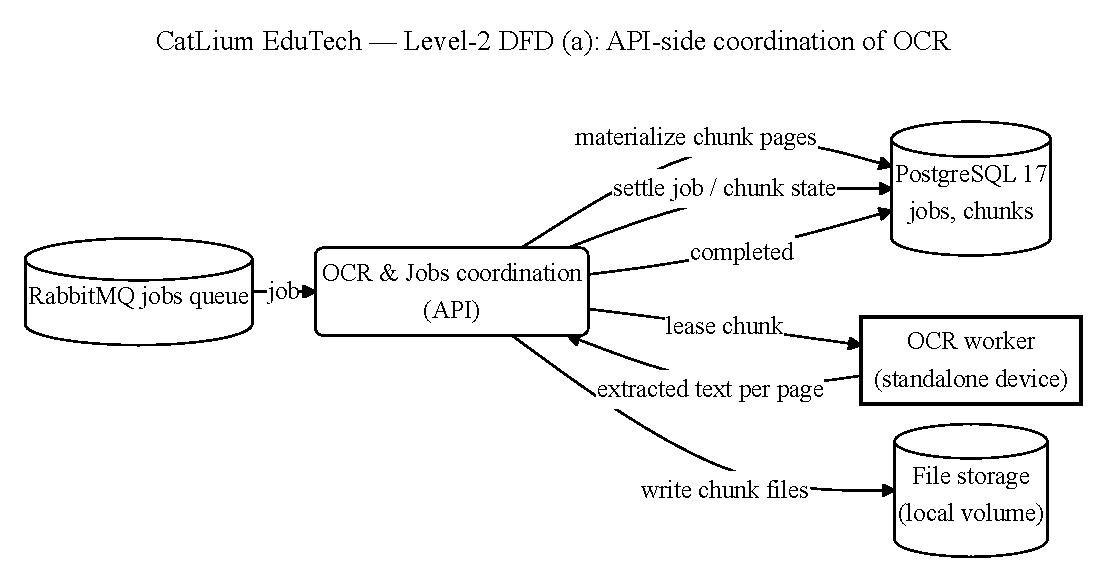
\includegraphics[width=711.5pt]{figures/dfd-level2a-coordination-bw.pdf}
\caption{Level-2 data flow diagram --- OCR and material-processing pipeline,
part 1: API-side coordination of chunk leasing, aggregation, and job
settlement.}

\end{sidewaysfigure}
\begin{sidewaysfigure}[p]
\centering
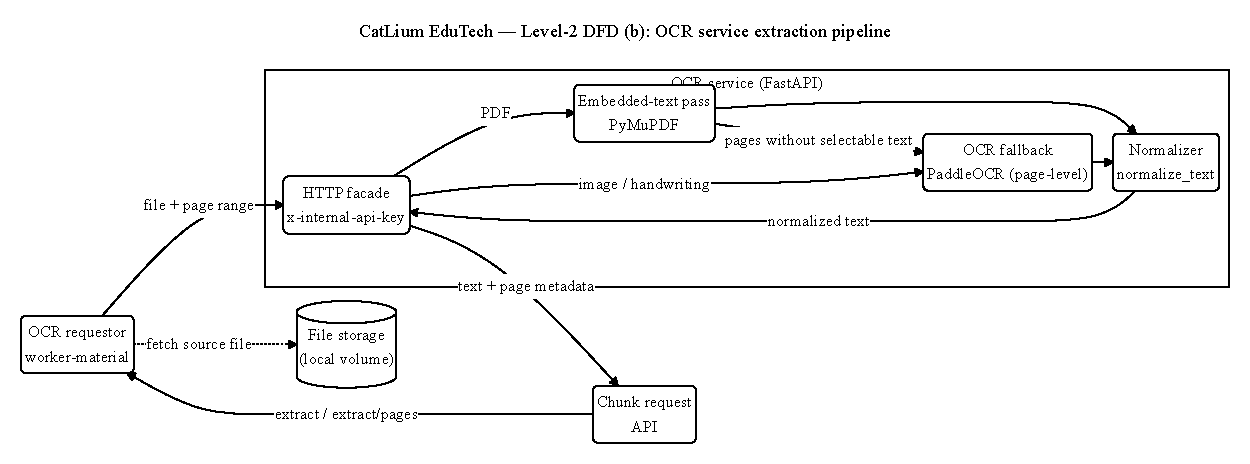
\includegraphics[width=711.5pt]{figures/dfd-level2b-ocrservice-bw.pdf}
\caption{Level-2 data flow diagram --- OCR and material-processing pipeline,
part 2: the OCR service extraction pipeline (embedded text, PaddleOCR
fallback, normalization).}

\end{sidewaysfigure}
\begin{figure}[htbp]
\centering
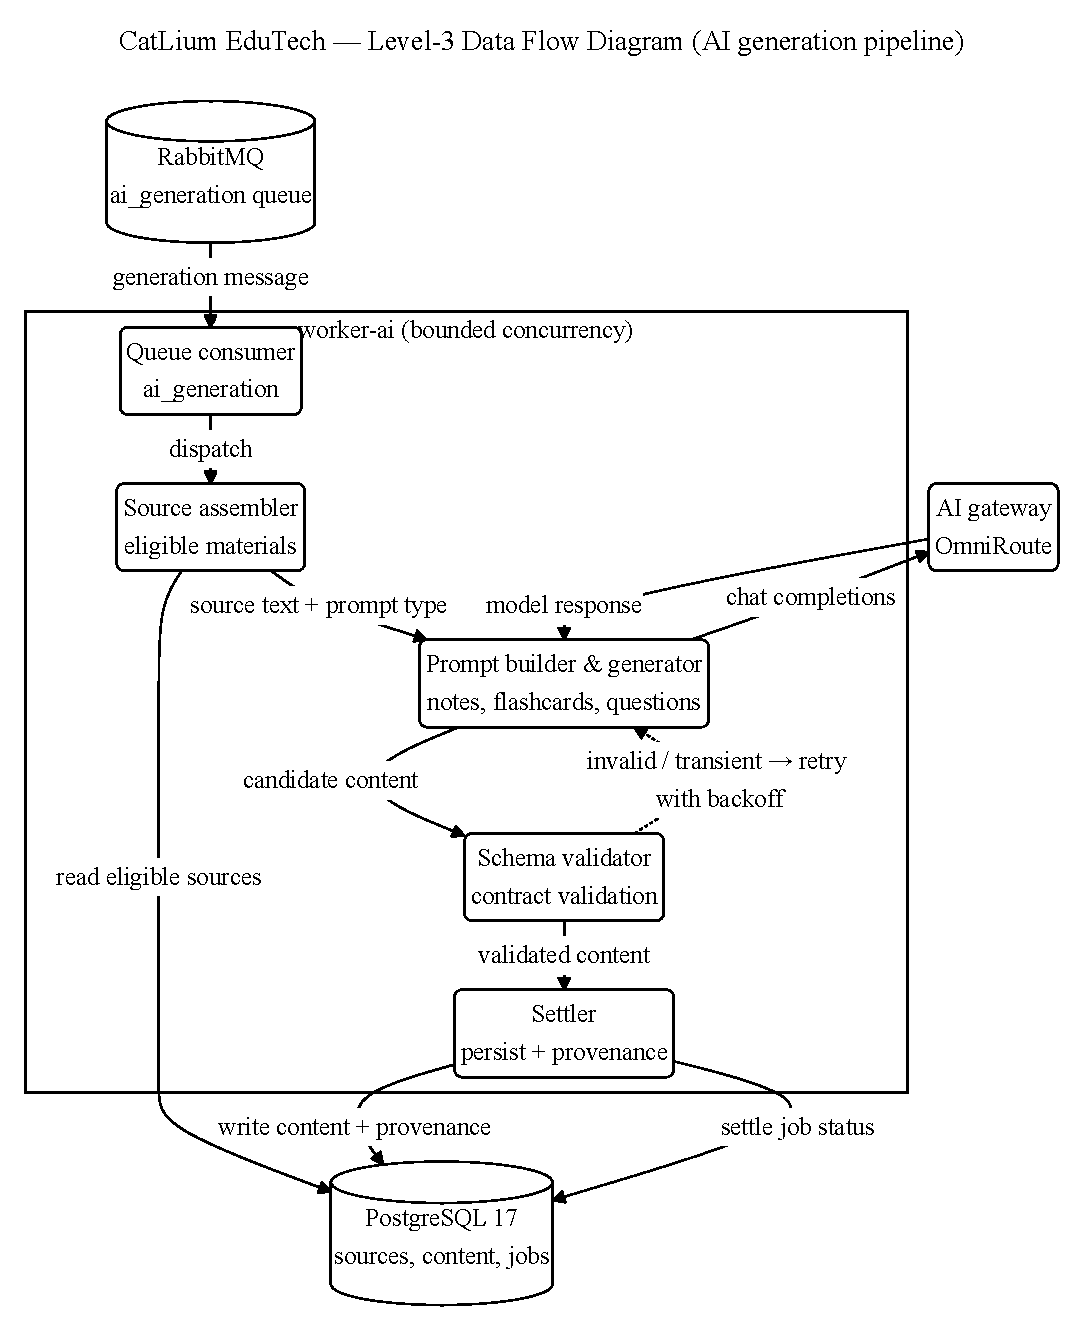
\includegraphics[width=425pt]{figures/dfd-level3-bw.pdf}
\caption{Level-3 data flow diagram: the AI generation pipeline inside
\texttt{worker-ai}.}

\end{figure}

\chapter{Database Design}

\begin{sidewaysfigure}[p]
\centering
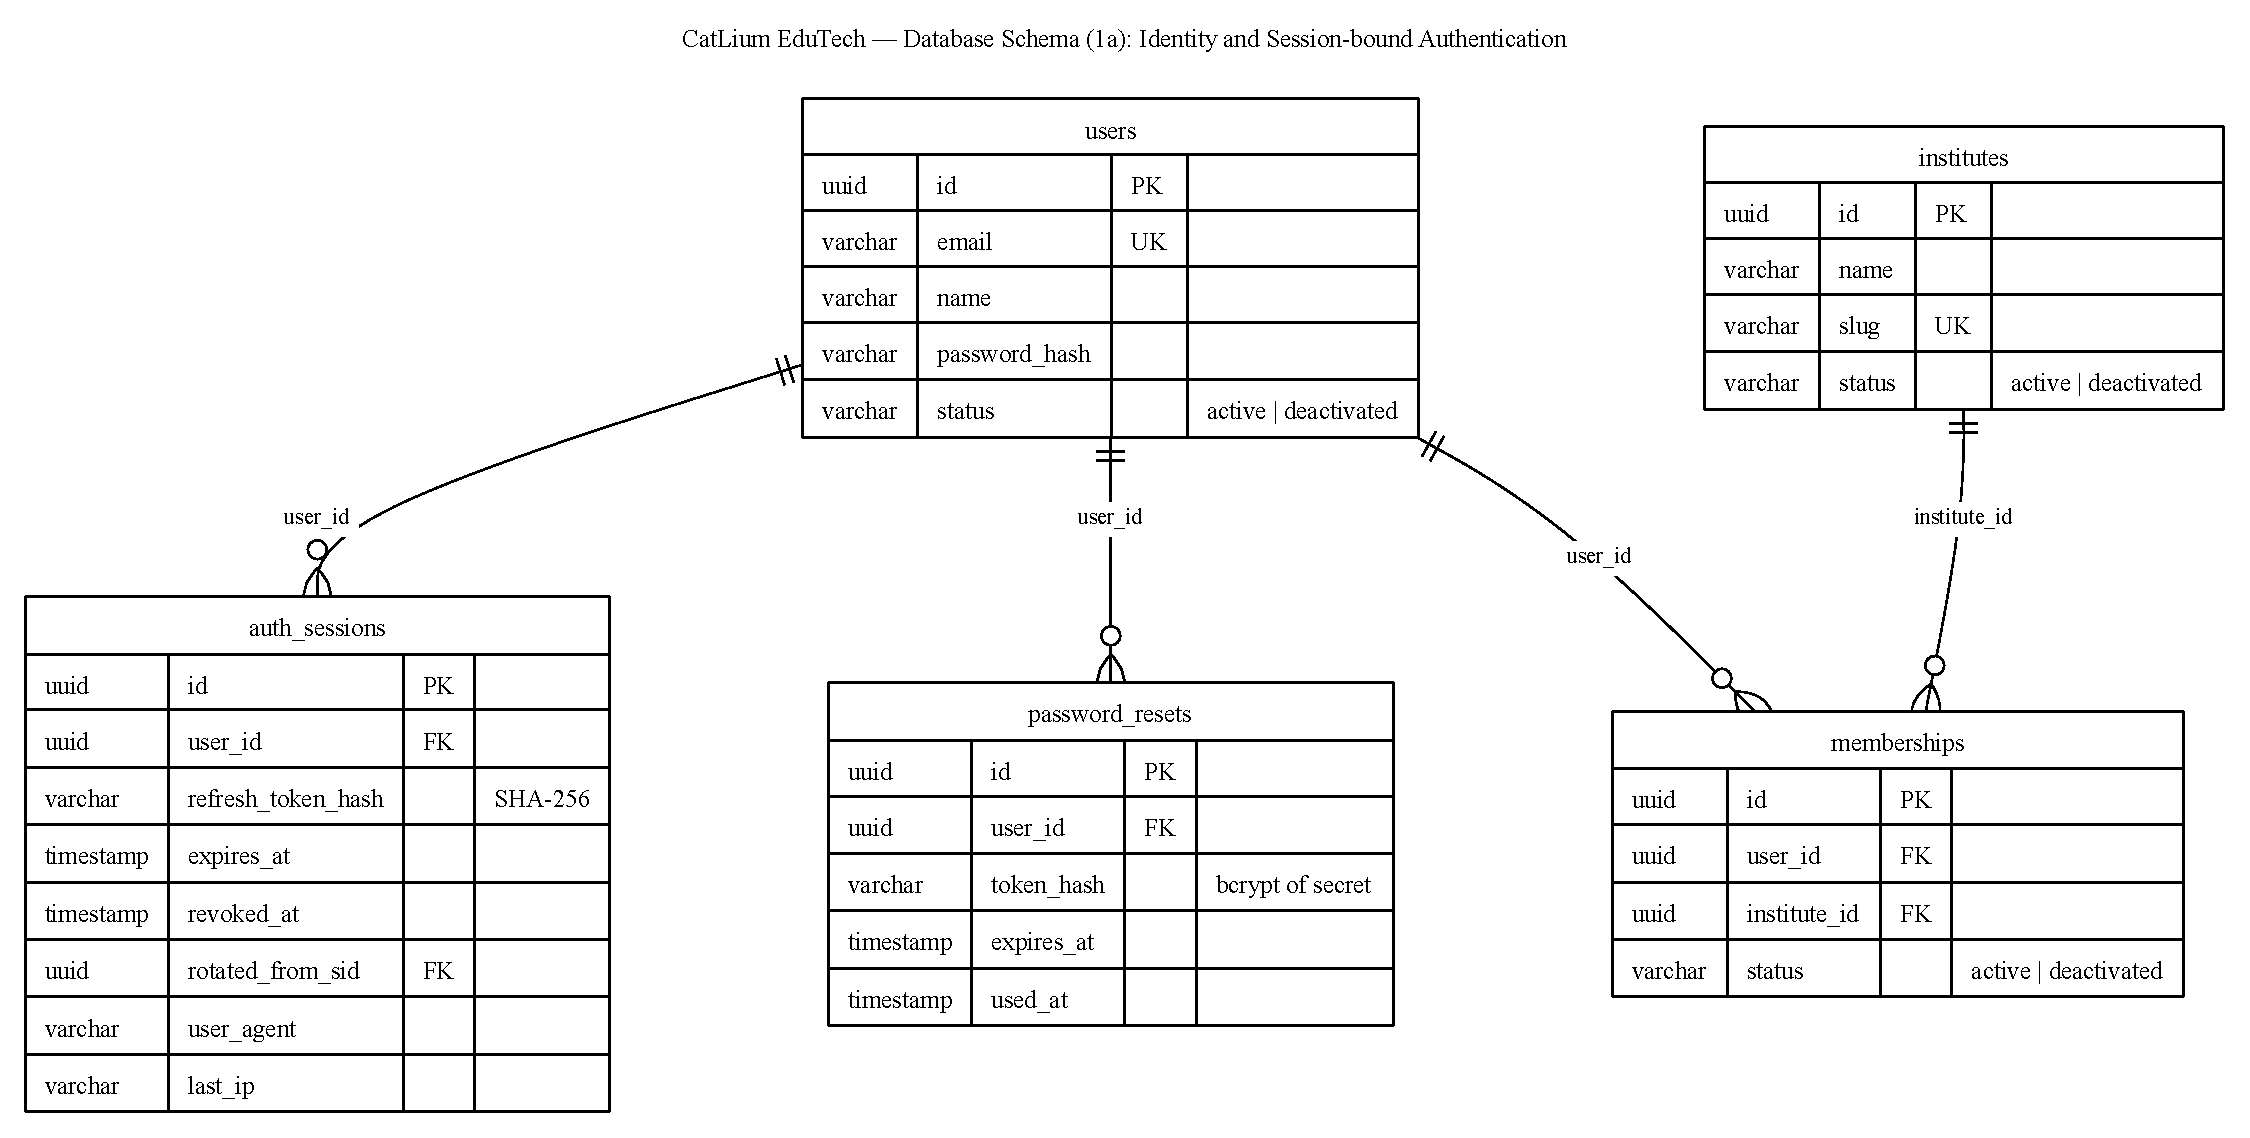
\includegraphics[width=711.5pt]{figures/erd-identity-auth-bw.pdf}
\caption{Database schema --- the identity and authentication core: users,
institute memberships, sessions, and password resets.}

\end{sidewaysfigure}
\begin{sidewaysfigure}[p]
\centering
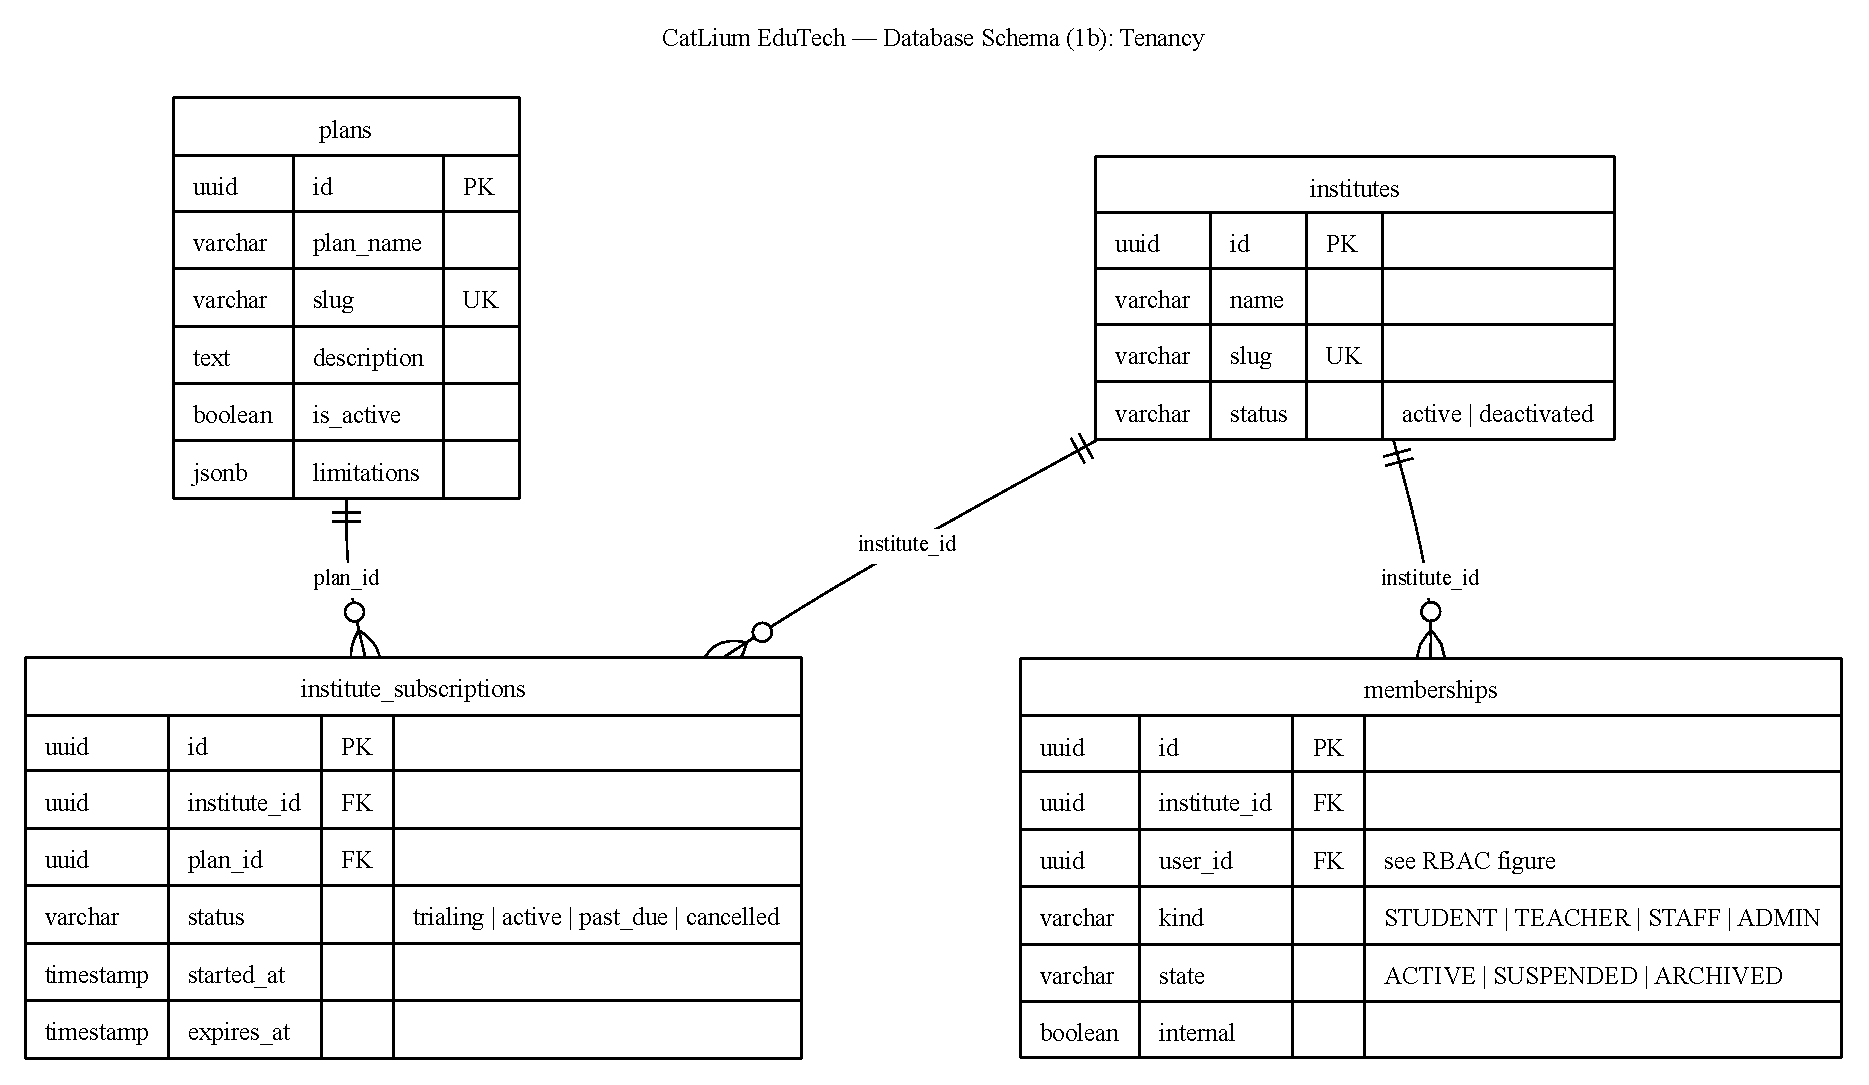
\includegraphics[width=689.5pt]{figures/erd-tenancy-bw.pdf}
\caption{Database schema --- the tenancy core: institutes, memberships, and
subscription plans.}

\end{sidewaysfigure}
\begin{sidewaysfigure}[p]
\centering
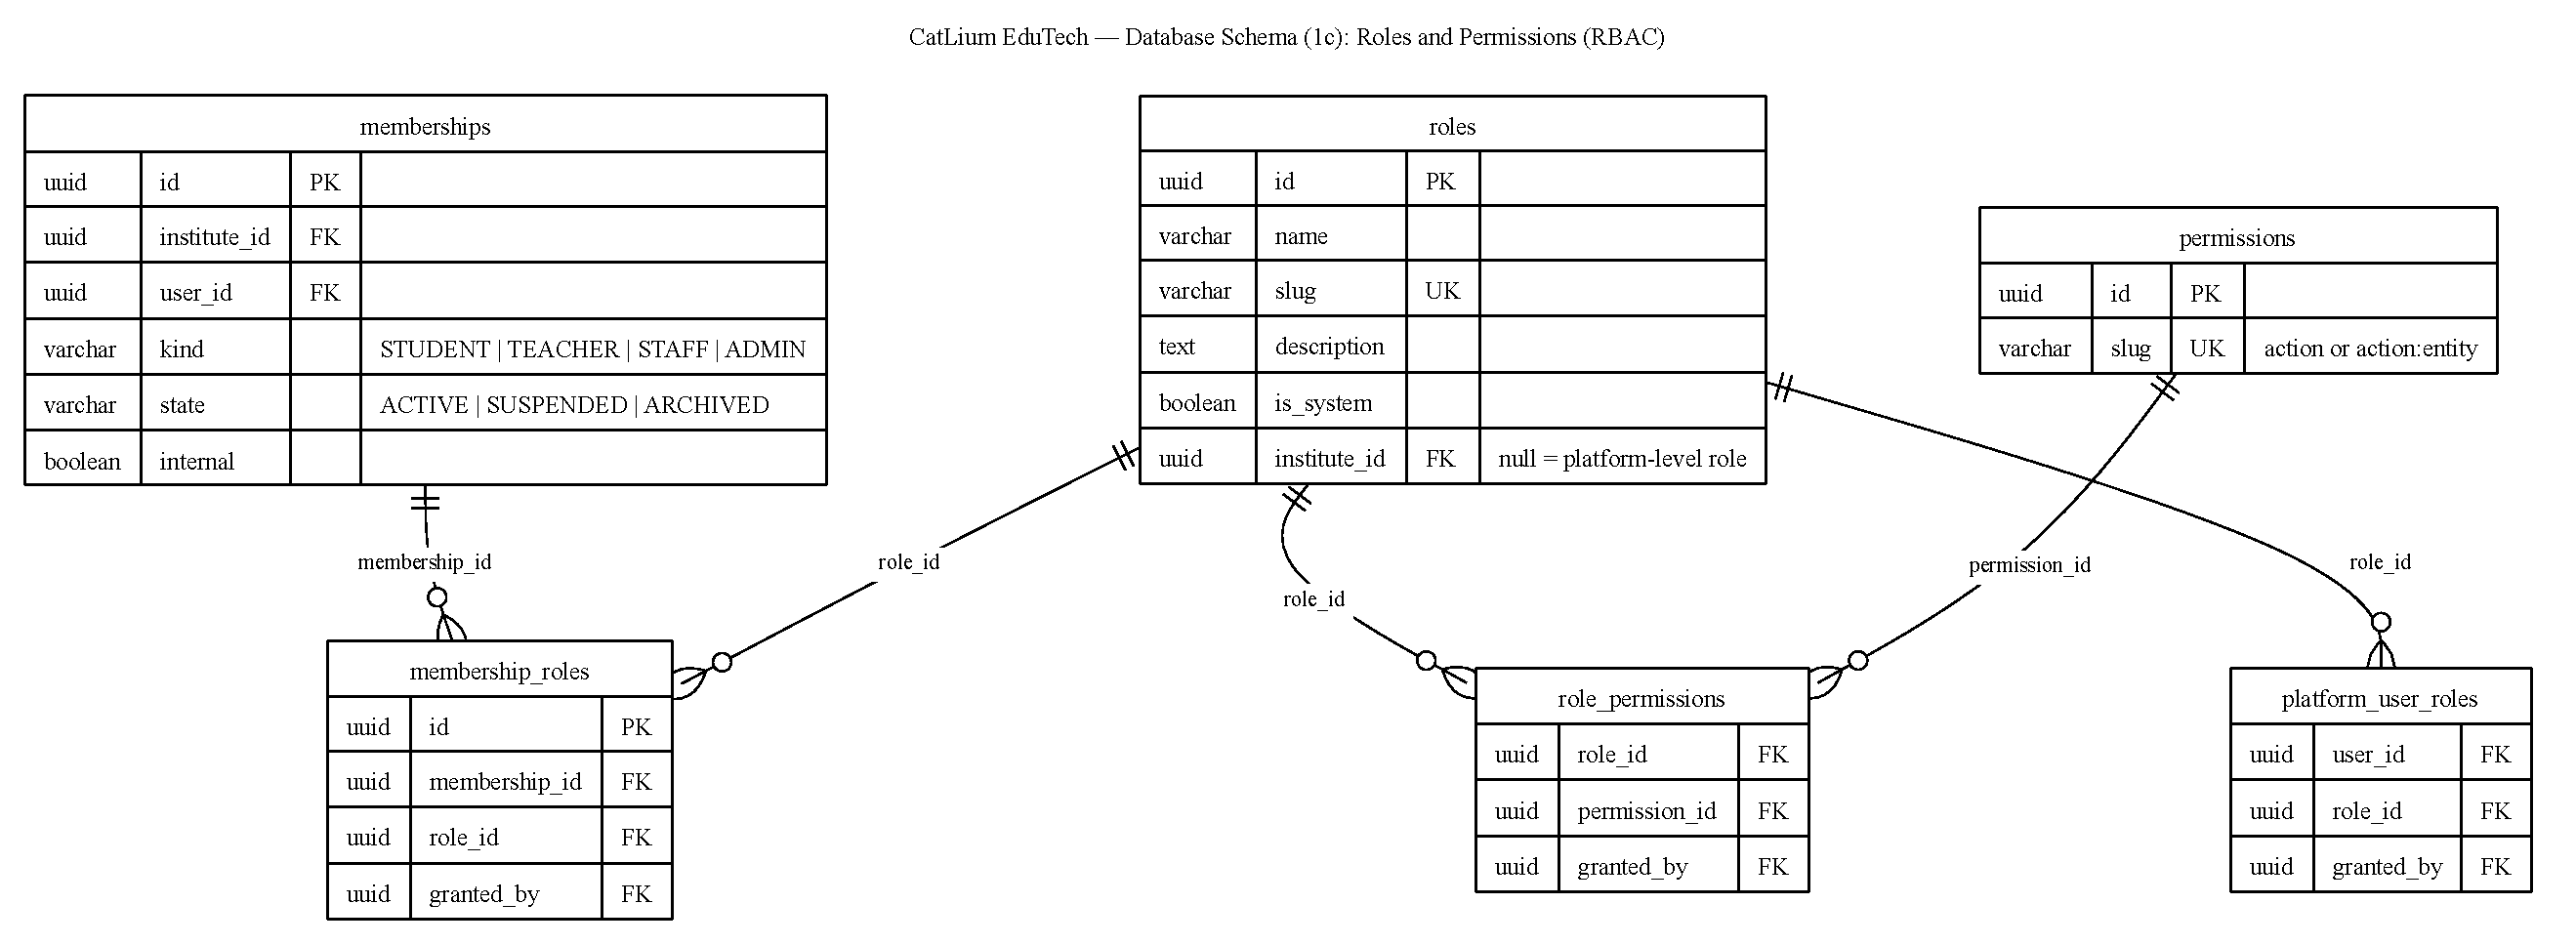
\includegraphics[width=711.5pt]{figures/erd-rbac-bw.pdf}
\caption{Database schema --- the roles/permissions (RBAC) core.}

\end{sidewaysfigure}
\begin{sidewaysfigure}[p]
\centering
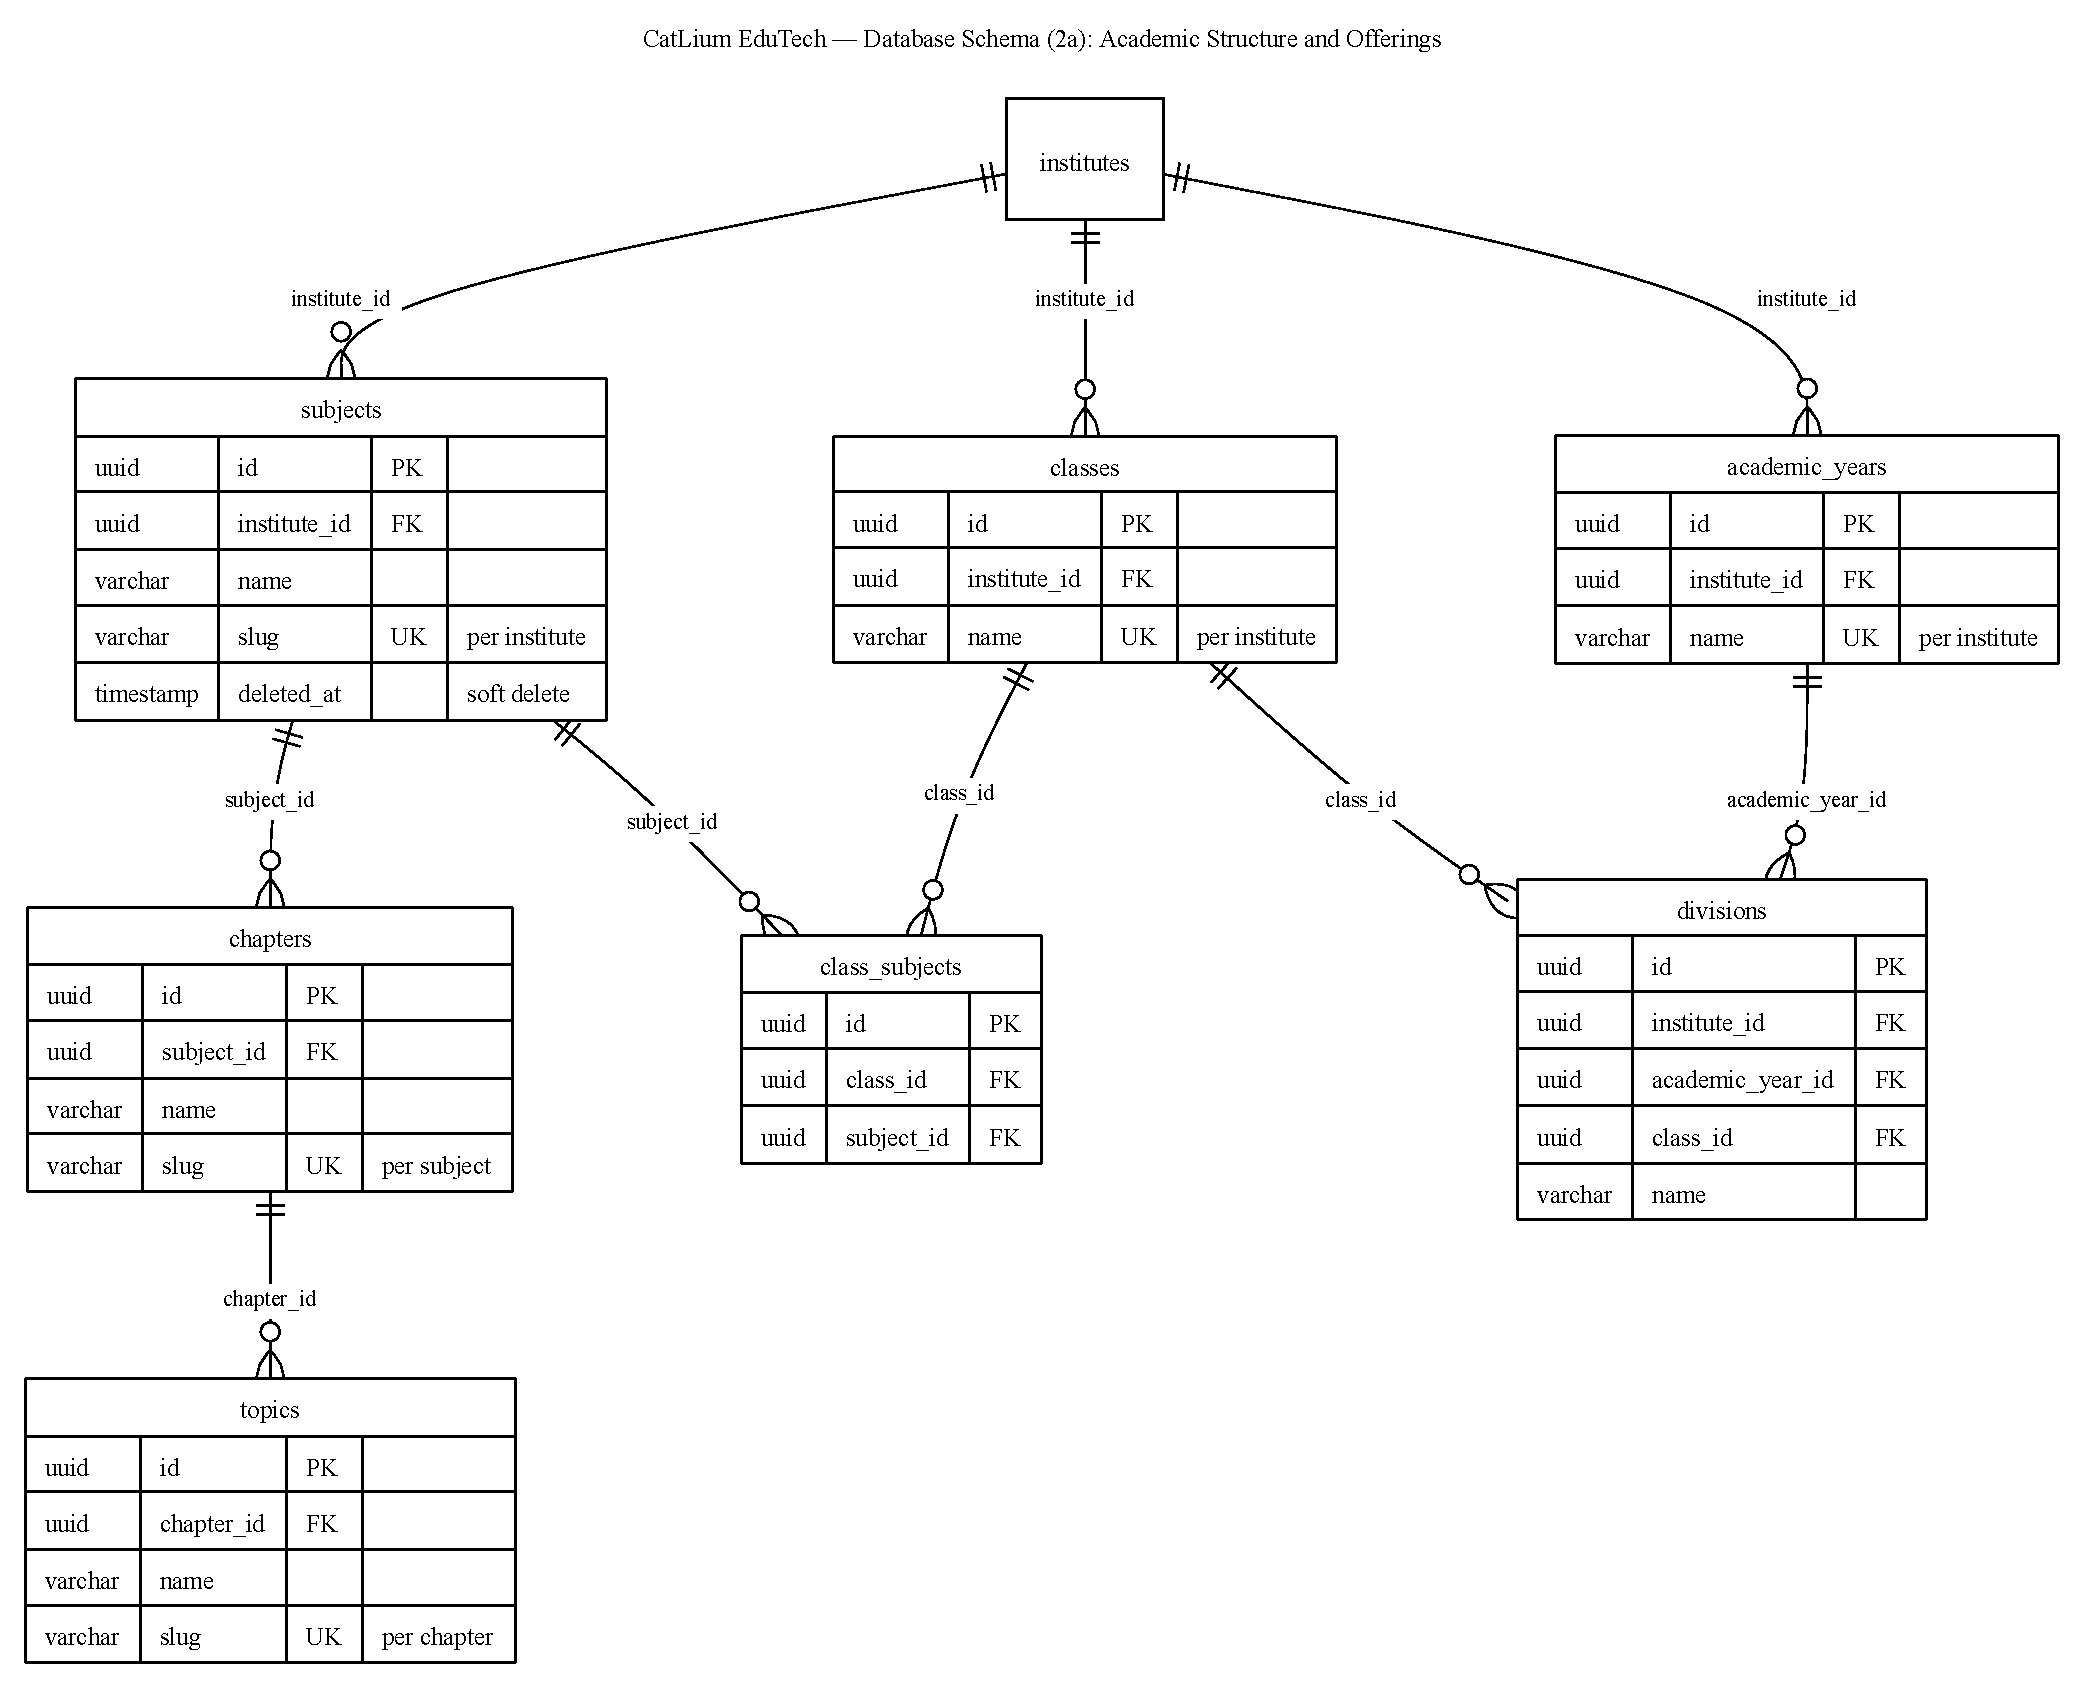
\includegraphics[width=494.9pt]{figures/erd-academic-structure-bw.pdf}
\caption{Database schema --- academic structure: the subject chain
($\texttt{subjects} \rightarrow \texttt{chapters} \rightarrow \texttt{topics}$),
class offerings, and academic years.}

\end{sidewaysfigure}
\begin{sidewaysfigure}[p]
\centering
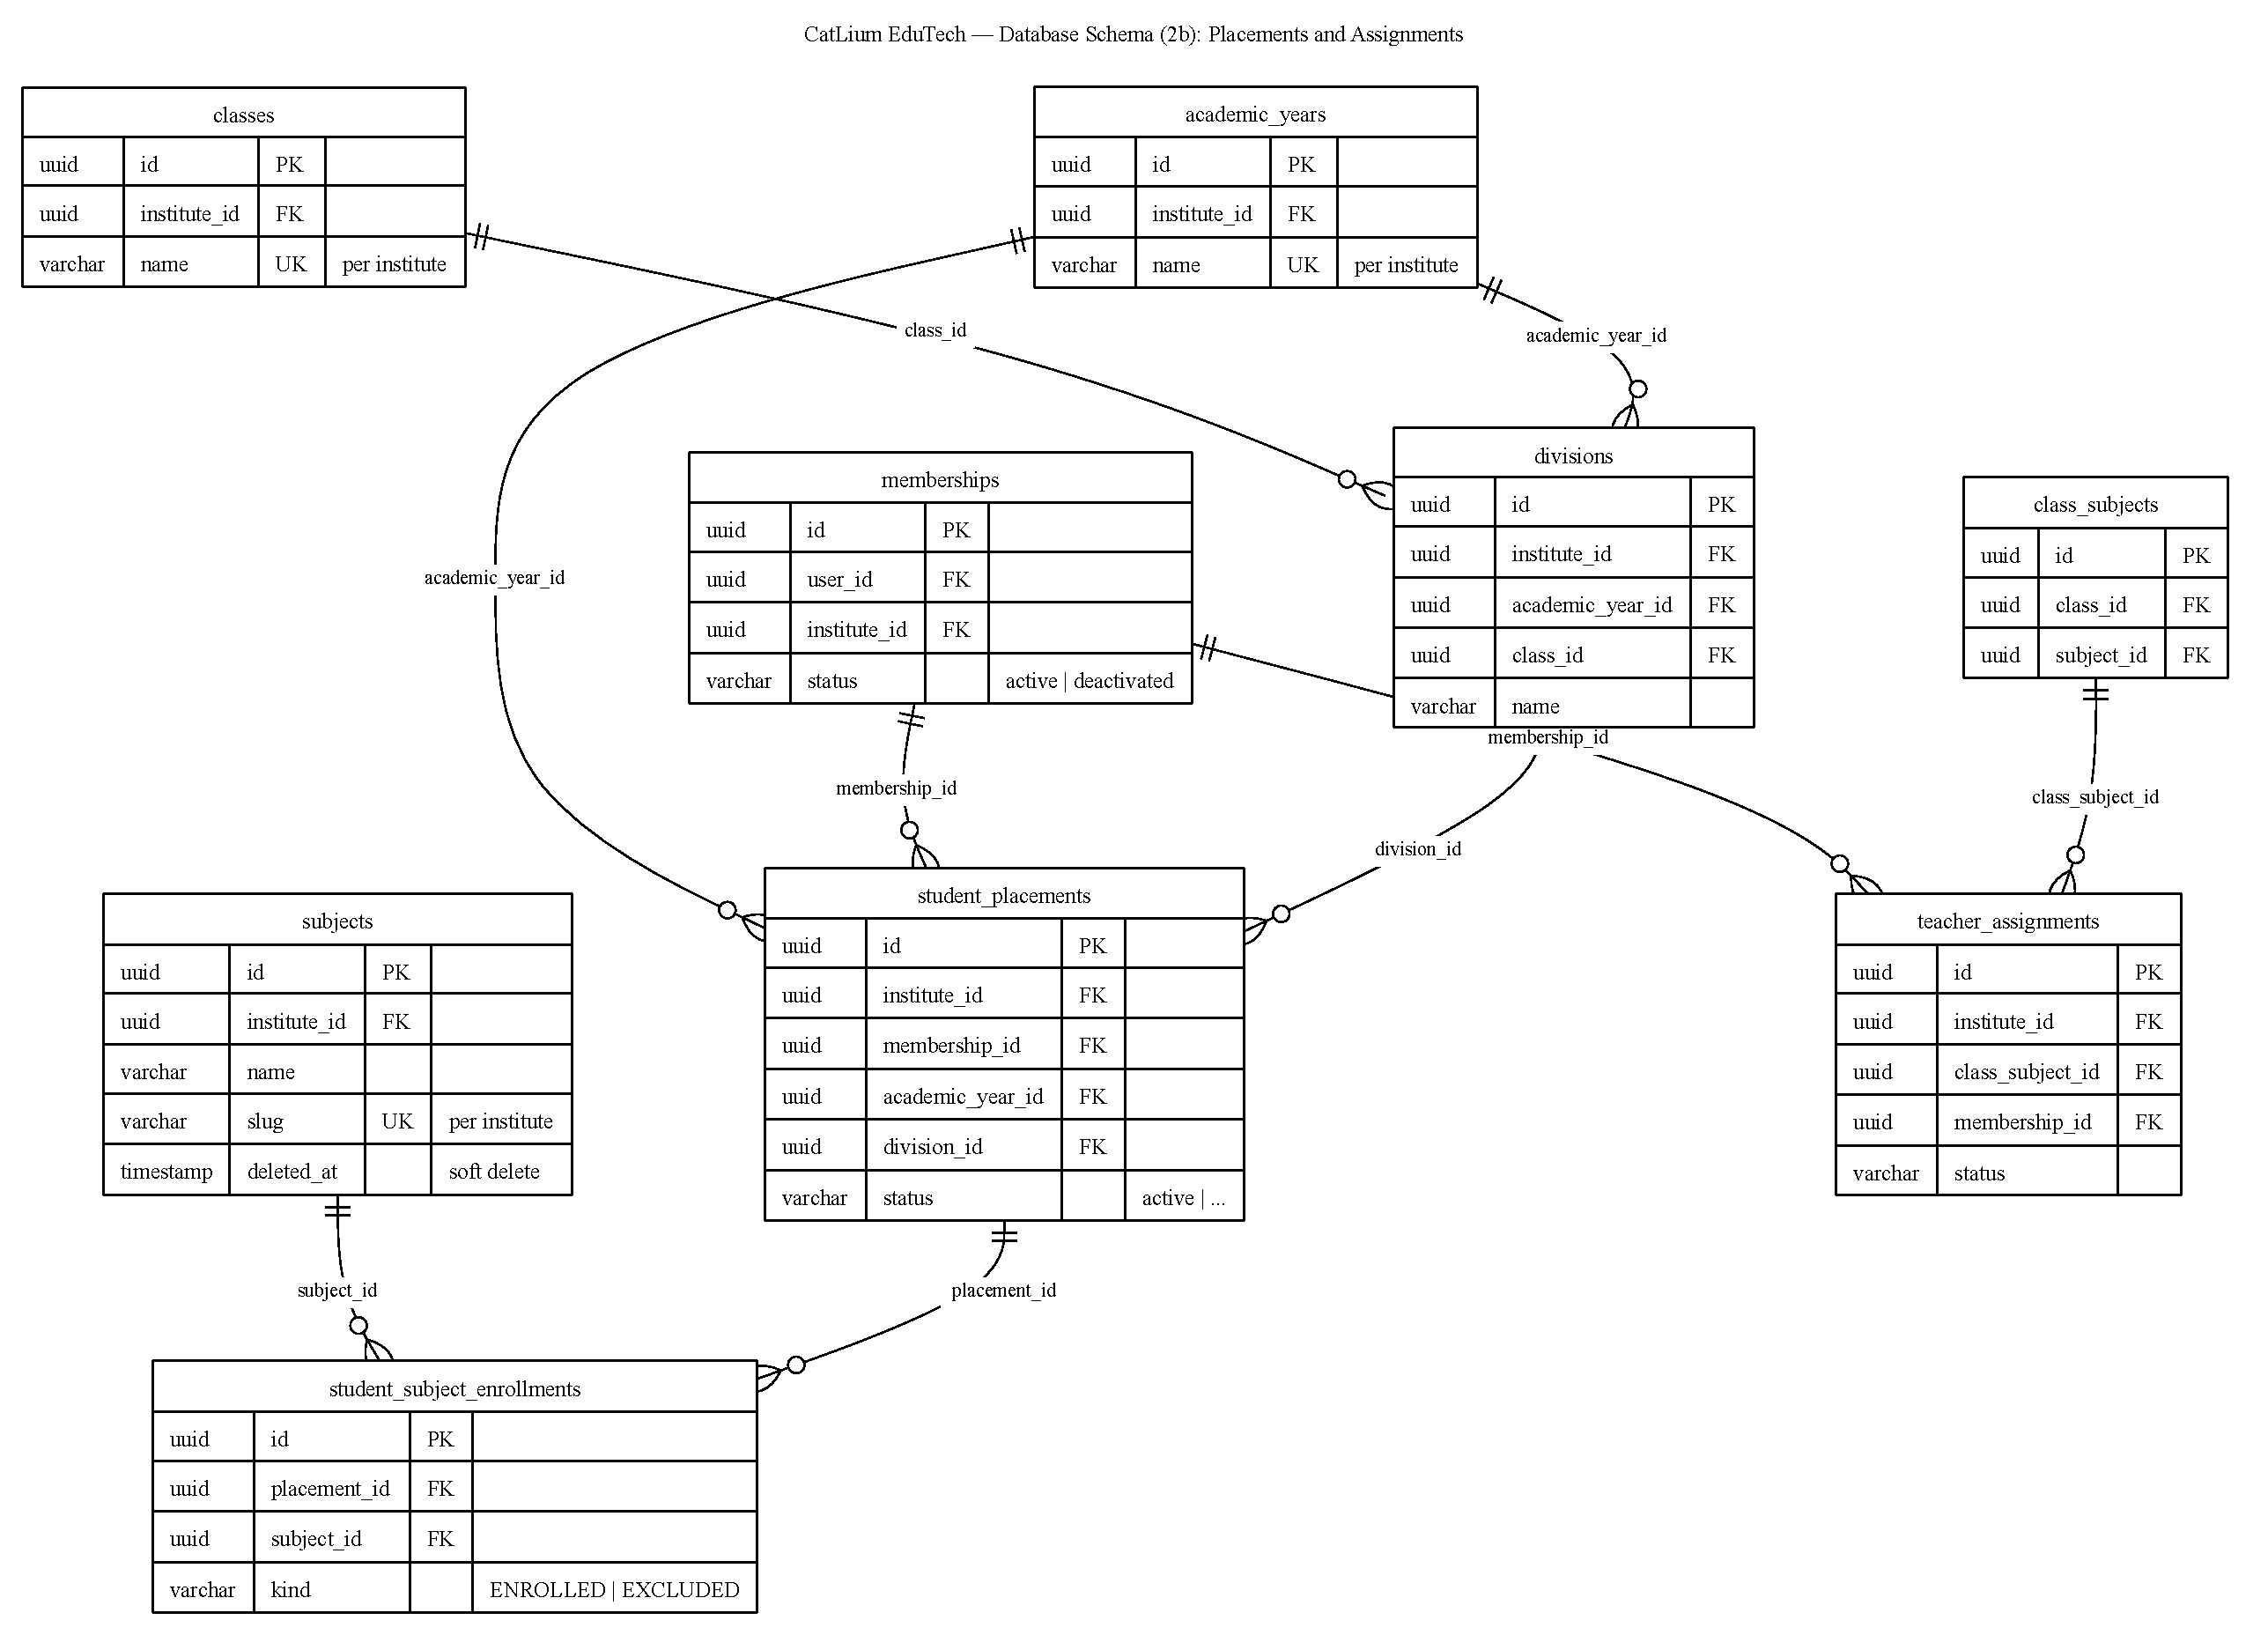
\includegraphics[width=555.6pt]{figures/erd-academic-placements-bw.pdf}
\caption{Database schema --- placements and assignments that derive the
academic scope for students and teachers.}

\end{sidewaysfigure}
\begin{figure}[p]
\centering
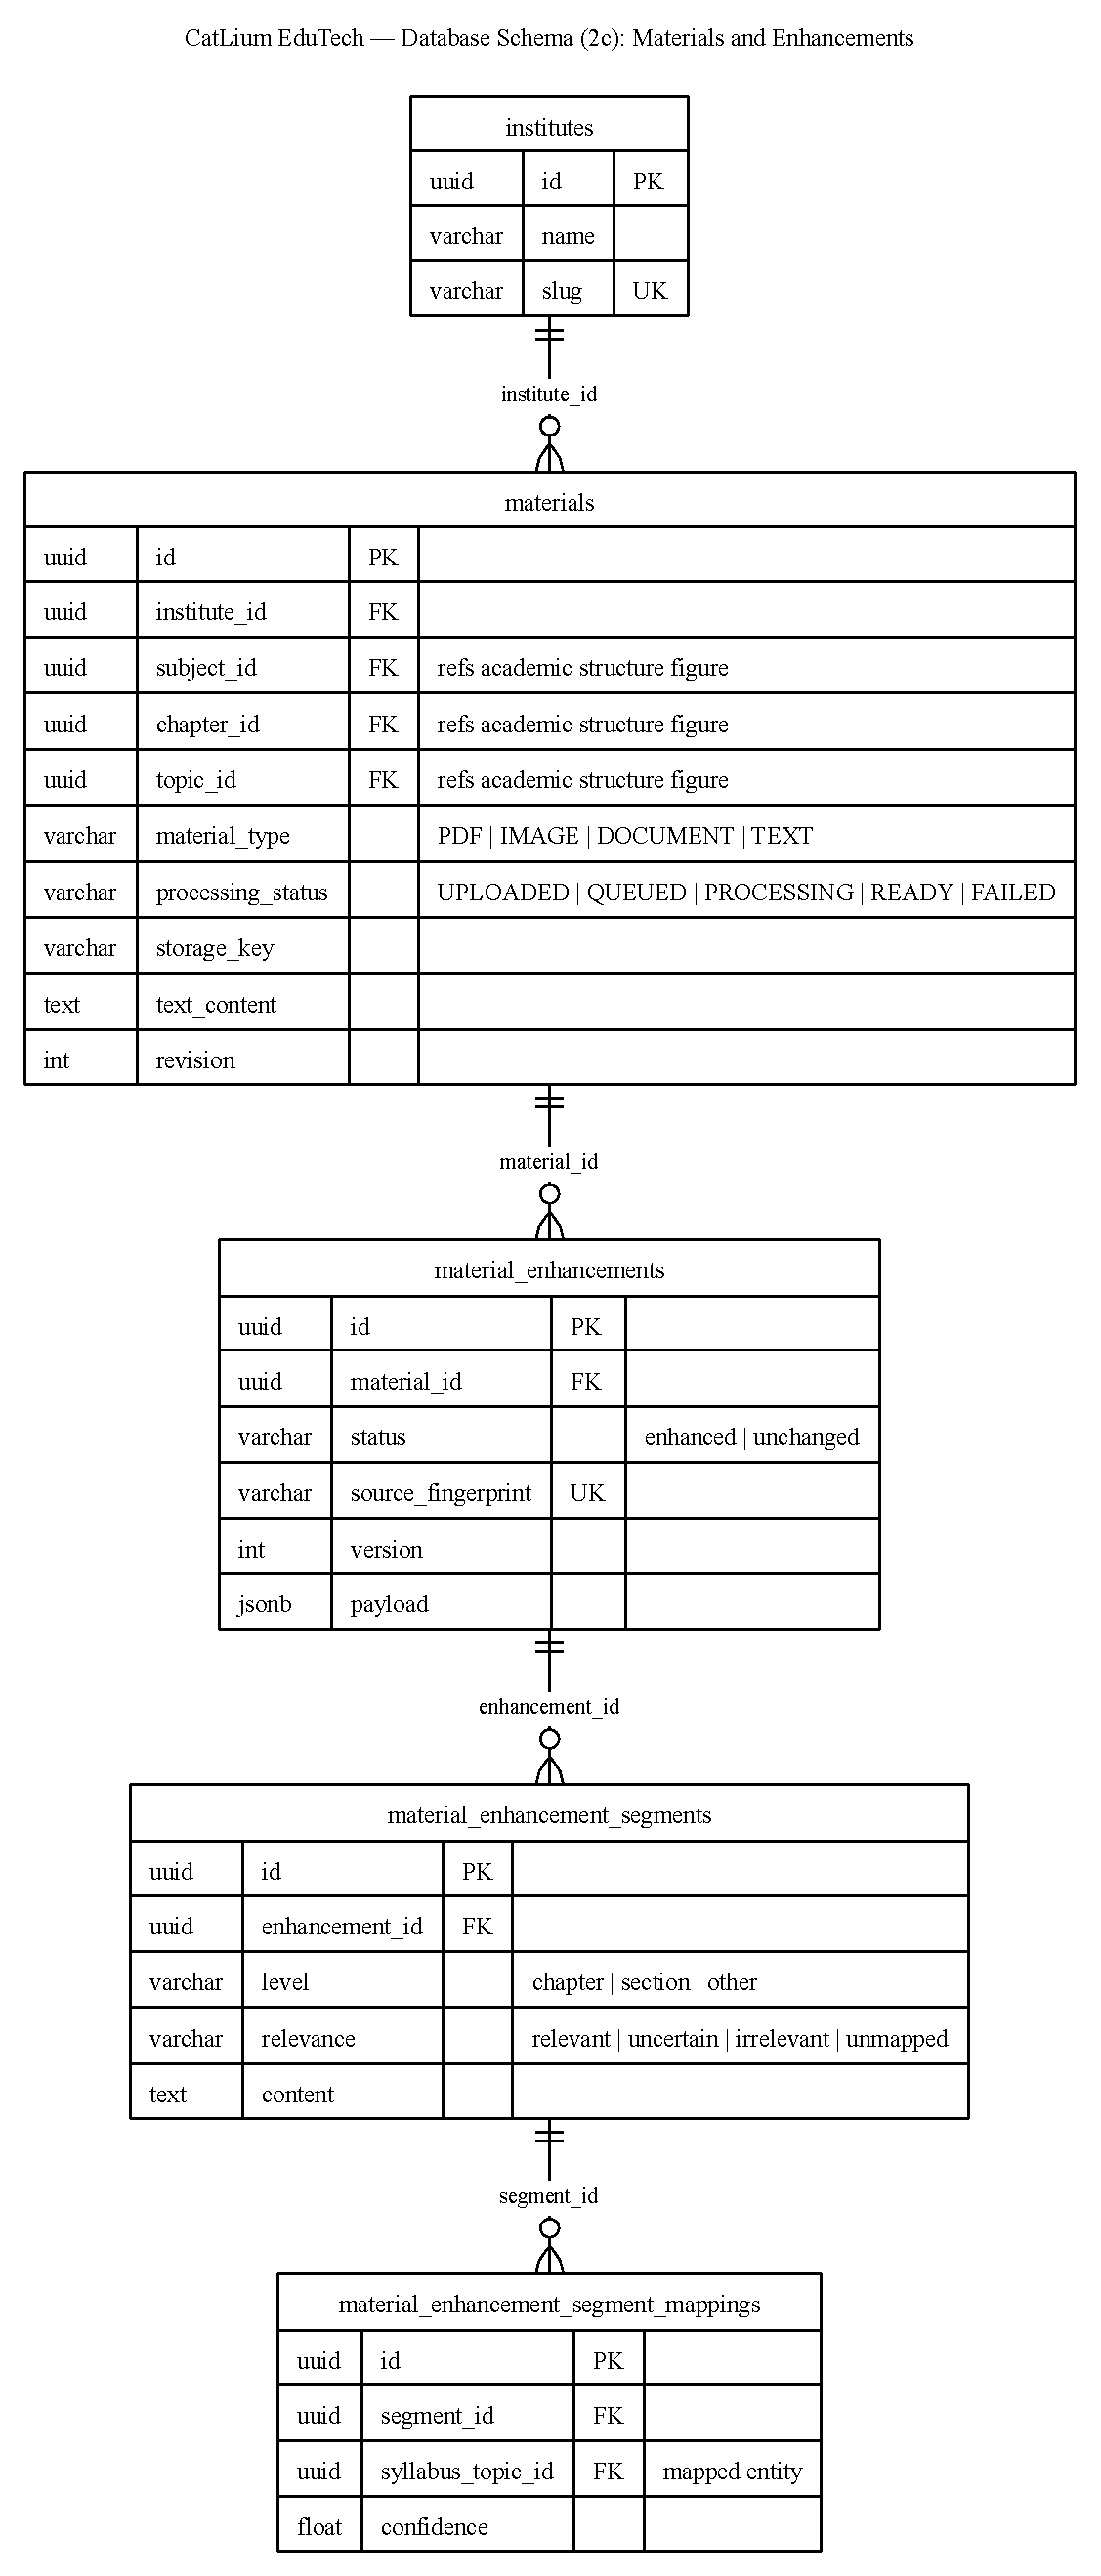
\includegraphics[width=290.6pt]{figures/erd-materials-enhancements-bw.pdf}
\caption{Database schema --- materials with their deterministic enhancement
chain.}

\end{figure}
\begin{figure}[p]
\centering
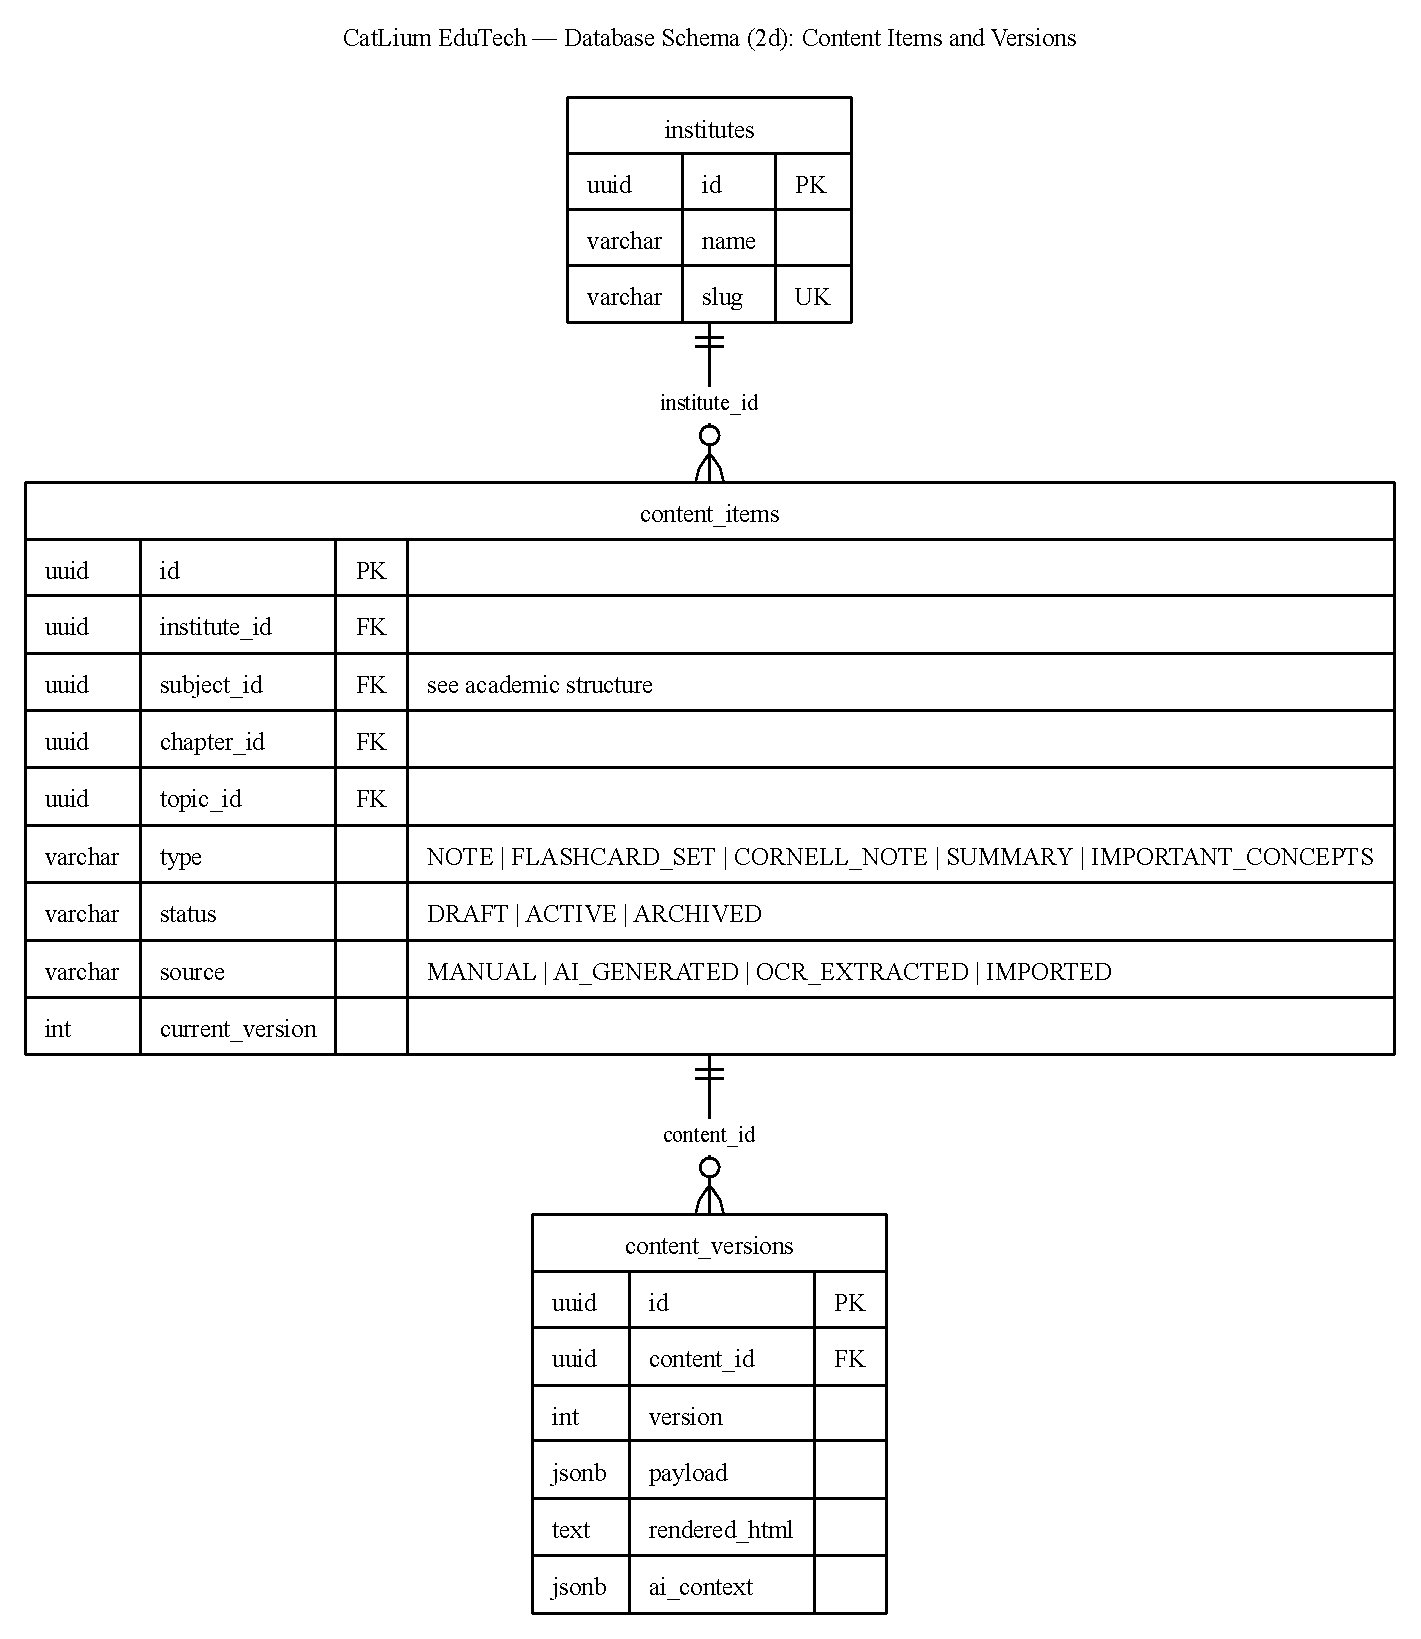
\includegraphics[width=436.5pt]{figures/erd-content-versions-bw.pdf}
\caption{Database schema --- versioned content items.}

\end{figure}
\begin{sidewaysfigure}[p]
\centering
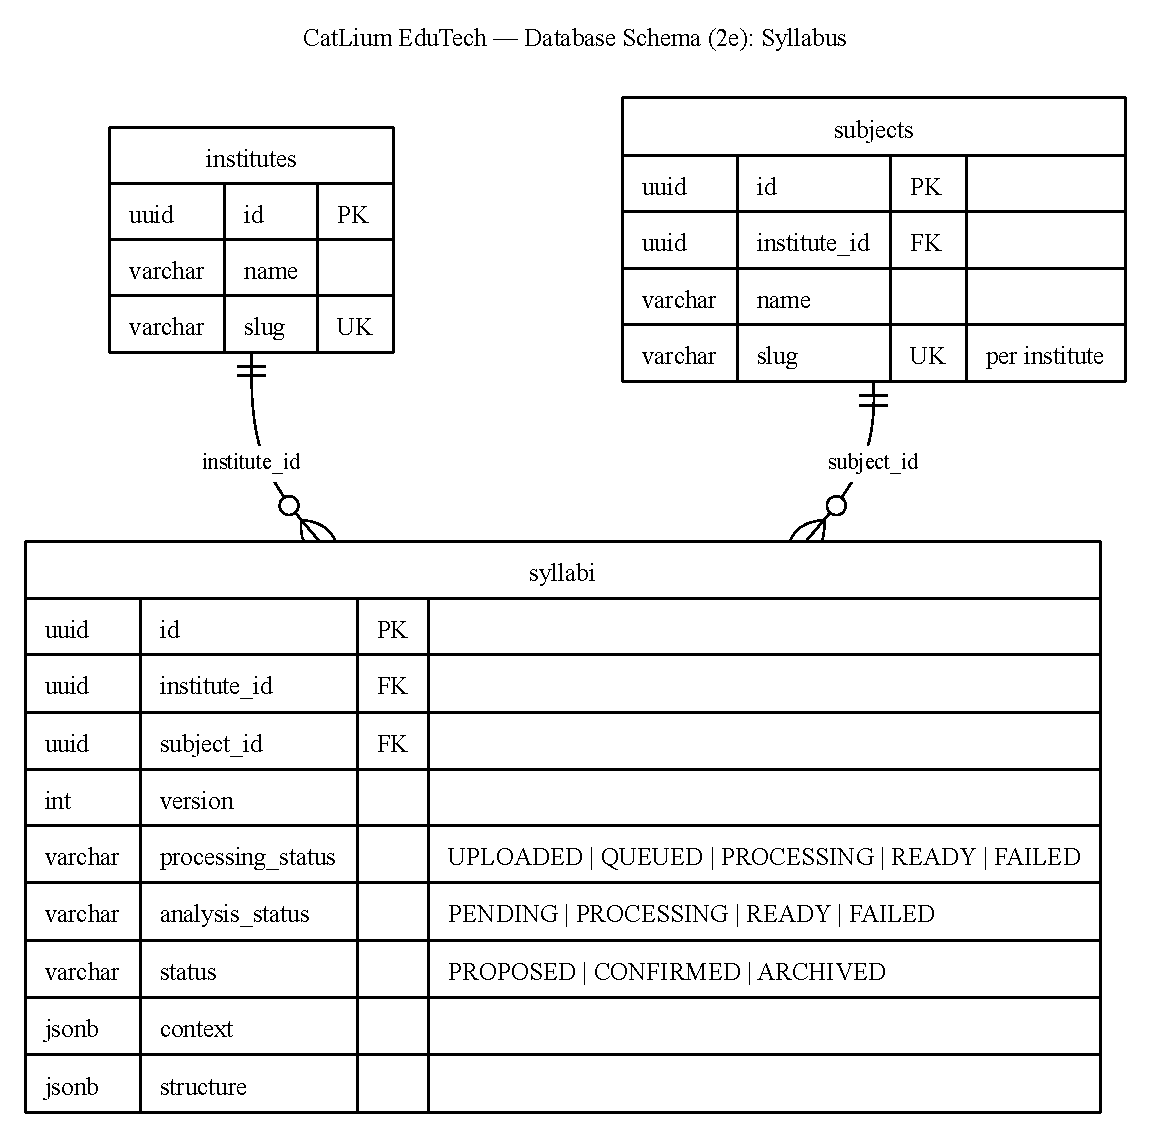
\includegraphics[width=404.9pt]{figures/erd-syllabus-bw.pdf}
\caption{Database schema --- per-subject syllabi and their lifecycle.}

\end{sidewaysfigure}
\begin{figure}[p]
\centering
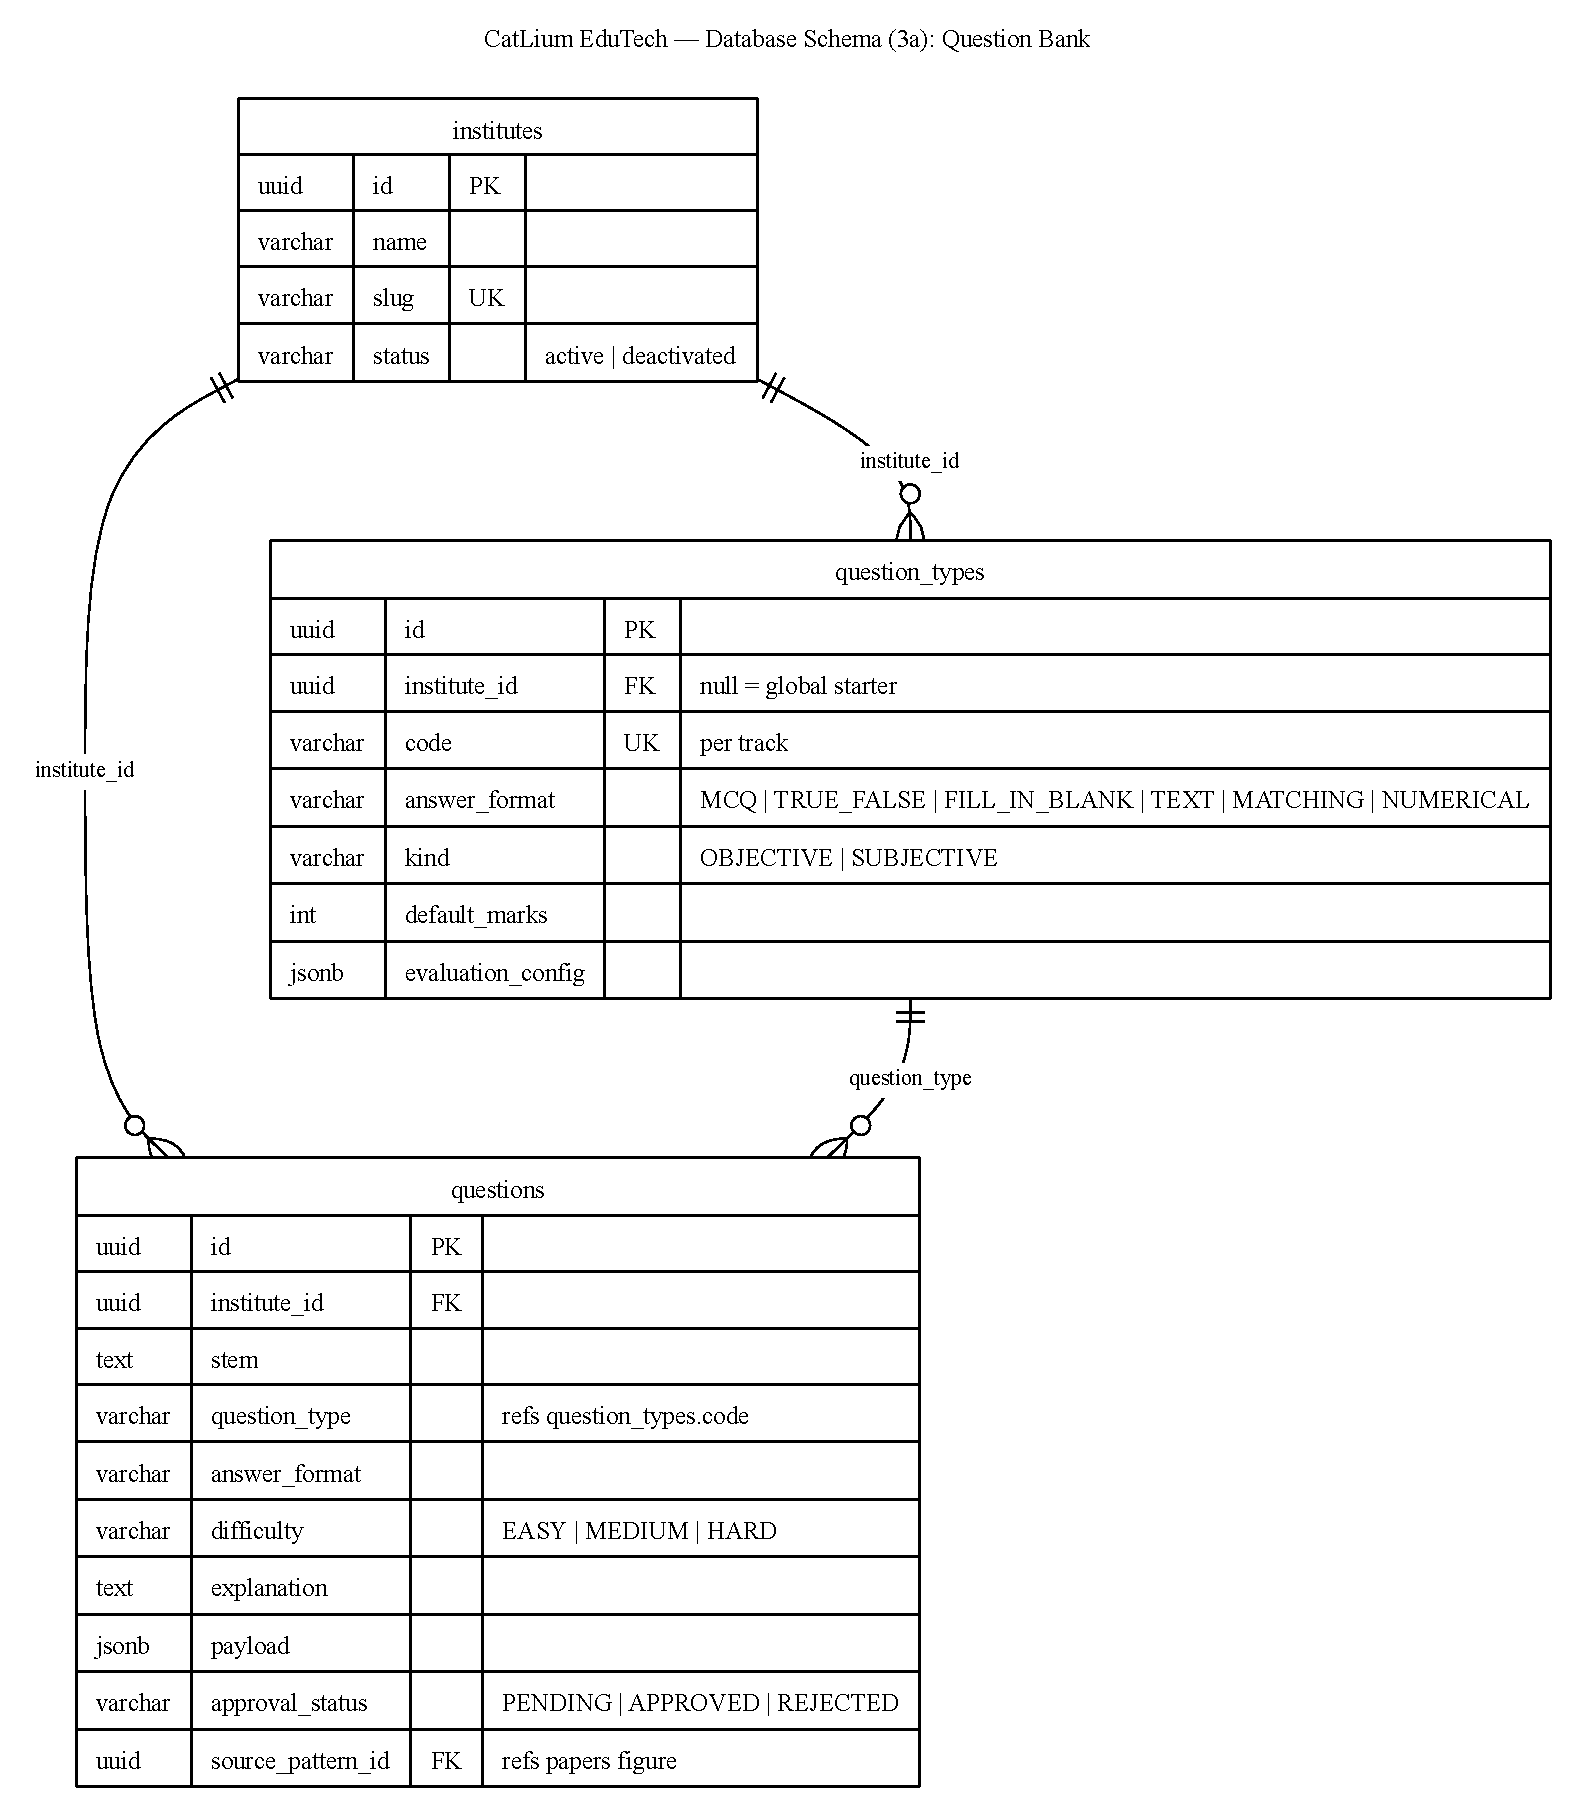
\includegraphics[width=436.5pt]{figures/erd-question-bank-bw.pdf}
\caption{Database schema --- question bank: question types and the scoped
\texttt{questions} table.}

\end{figure}
\begin{sidewaysfigure}[p]
\centering
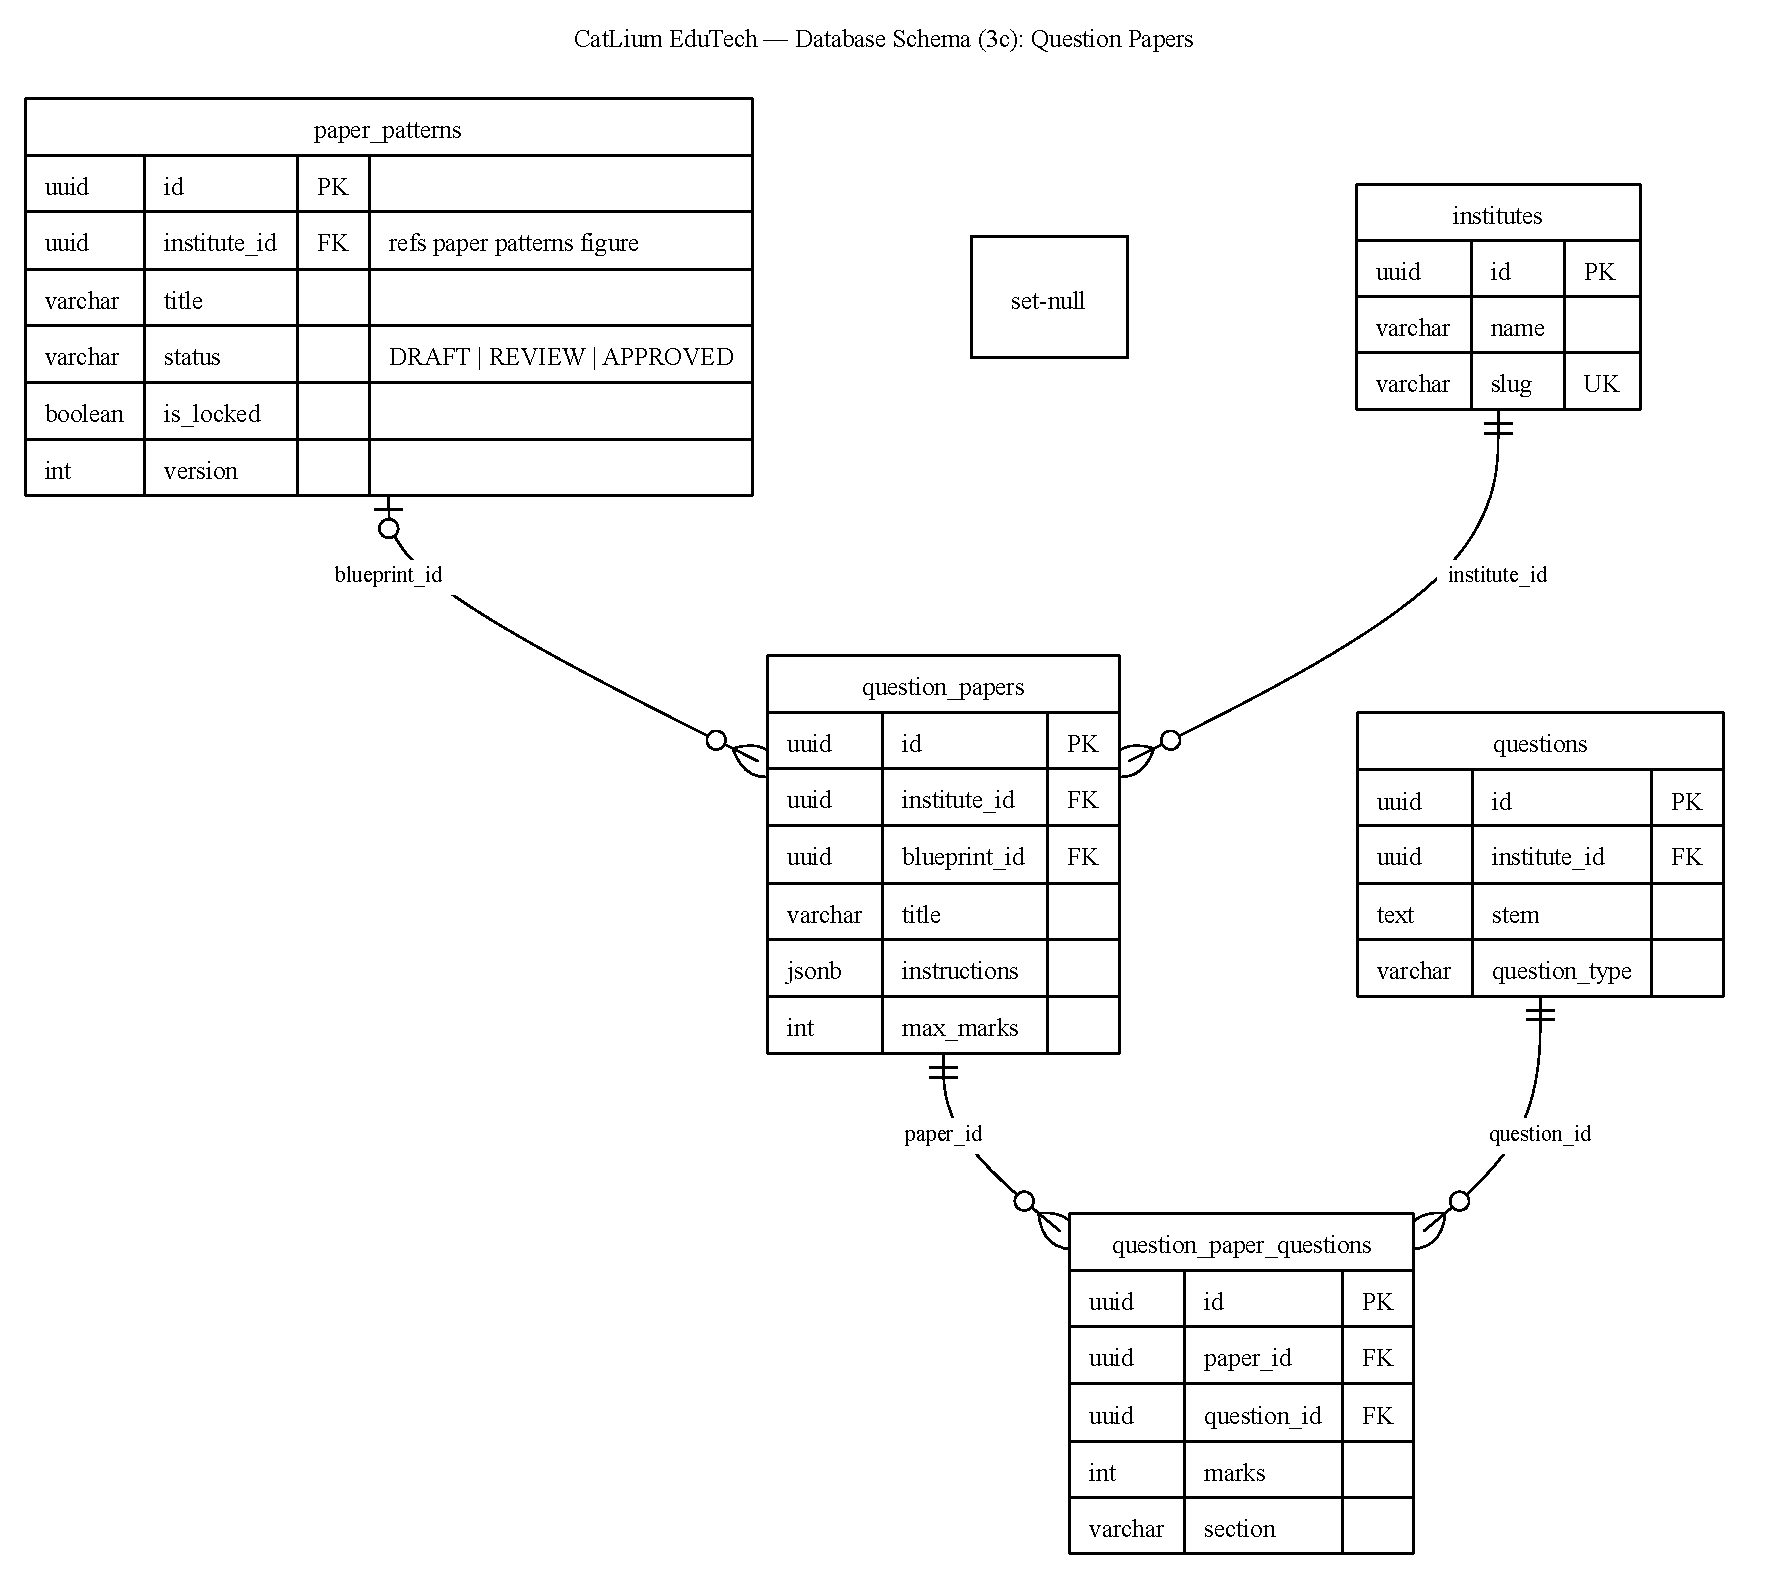
\includegraphics[width=448.6pt]{figures/erd-question-papers-bw.pdf}
\caption{Database schema --- question papers: the blueprint-driven
\texttt{question\_papers} snapshot.}

\end{sidewaysfigure}
\begin{sidewaysfigure}[p]
\centering
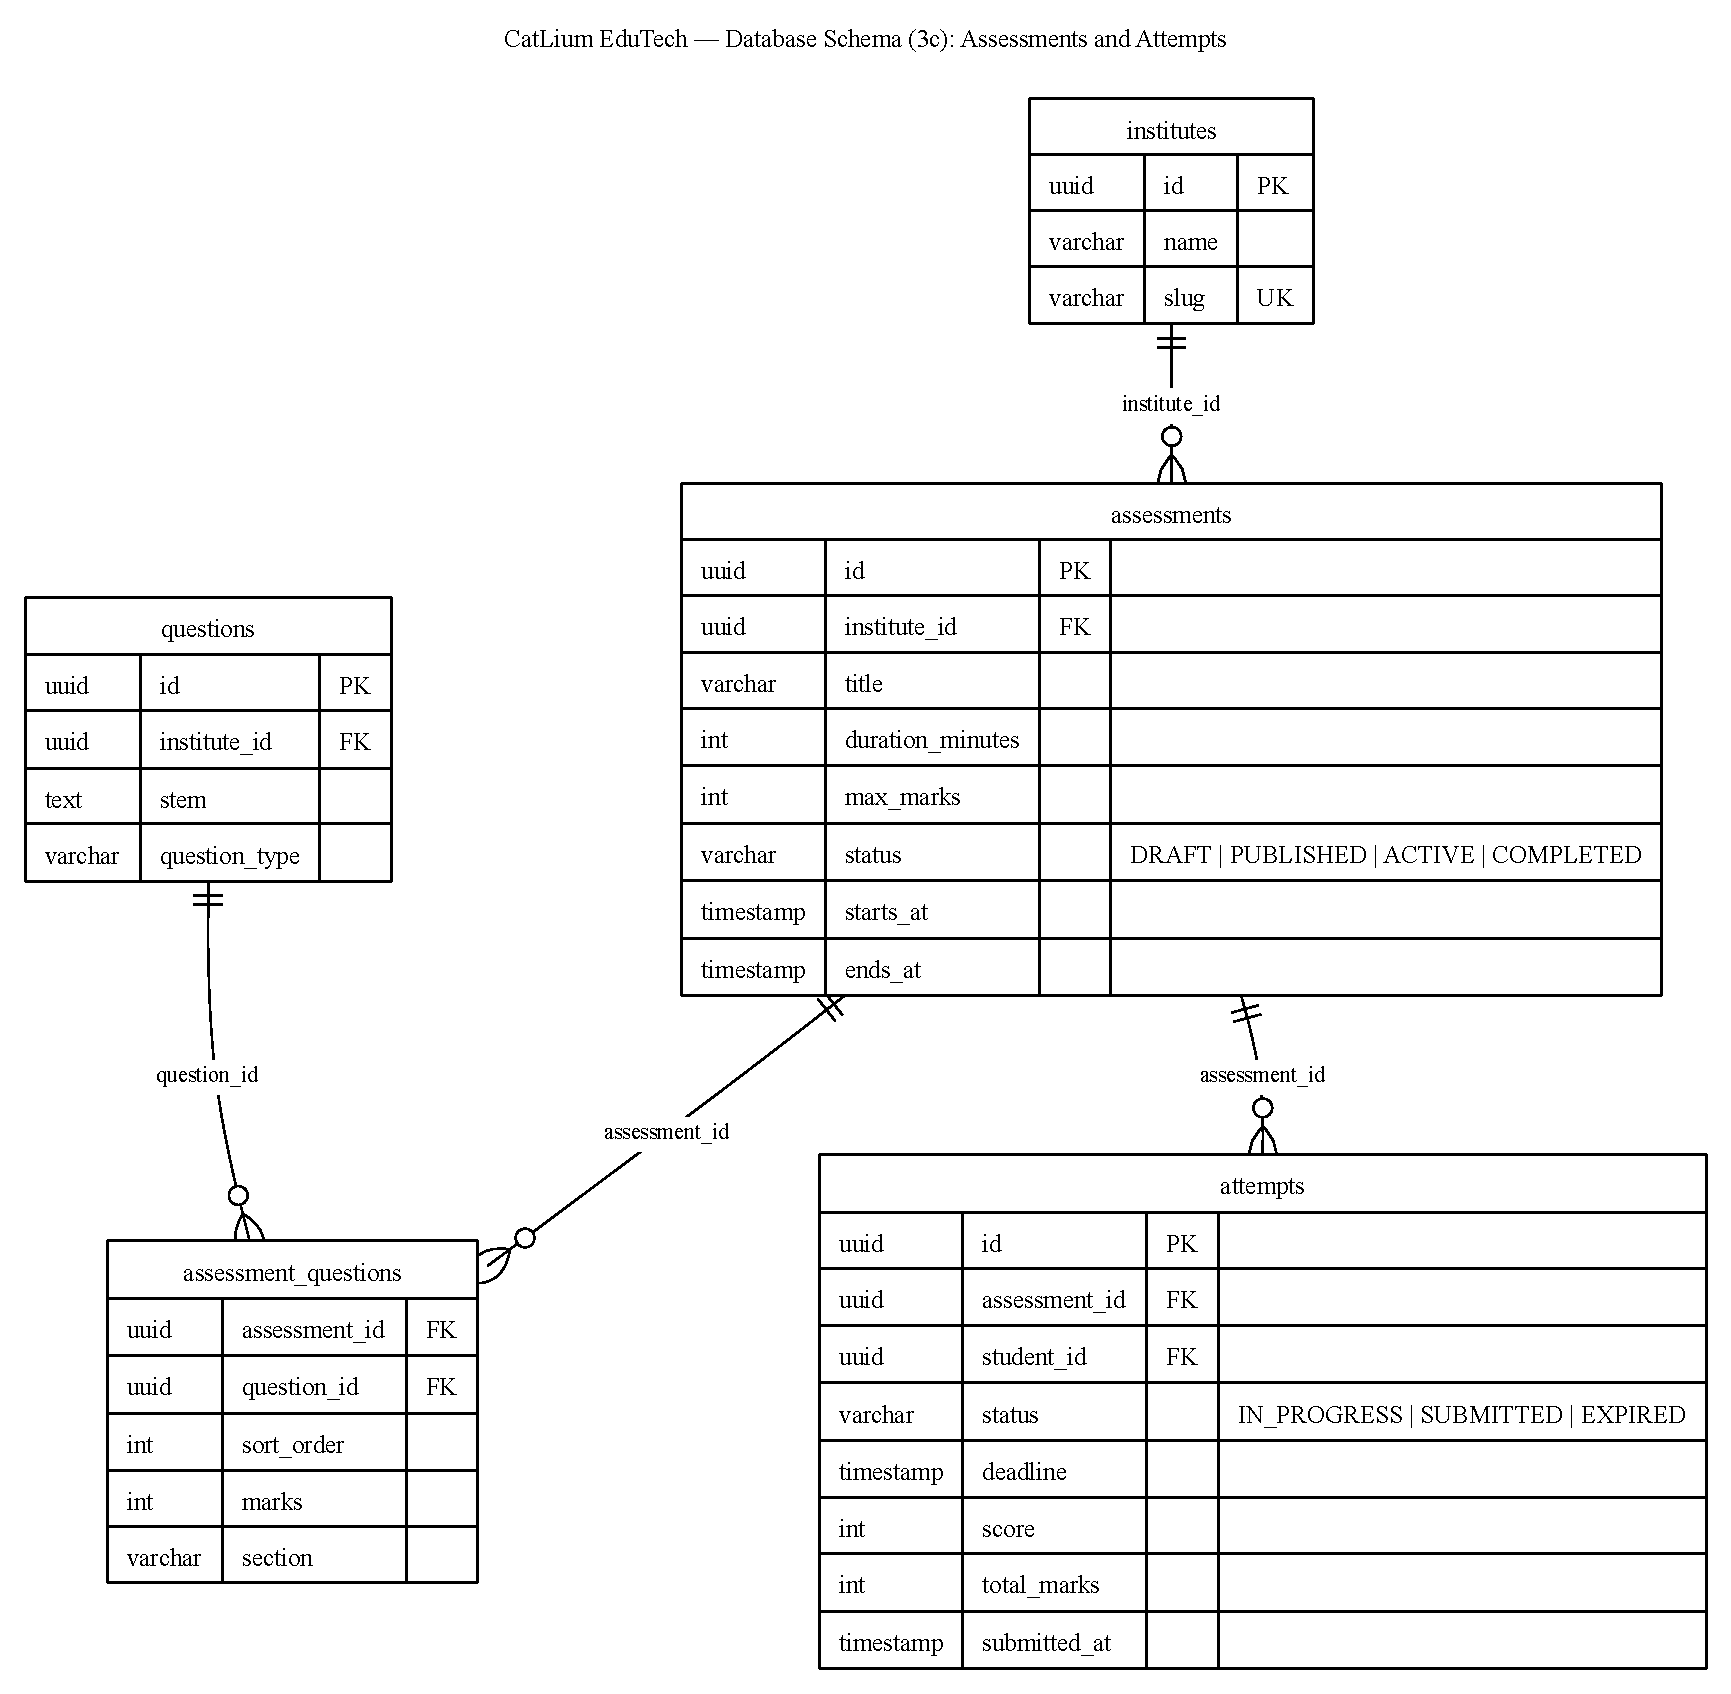
\includegraphics[width=409.4pt]{figures/erd-assessments-bw.pdf}
\caption{Database schema --- examination: assessments and their subject
binding.}

\end{sidewaysfigure}
\begin{figure}[p]
\centering
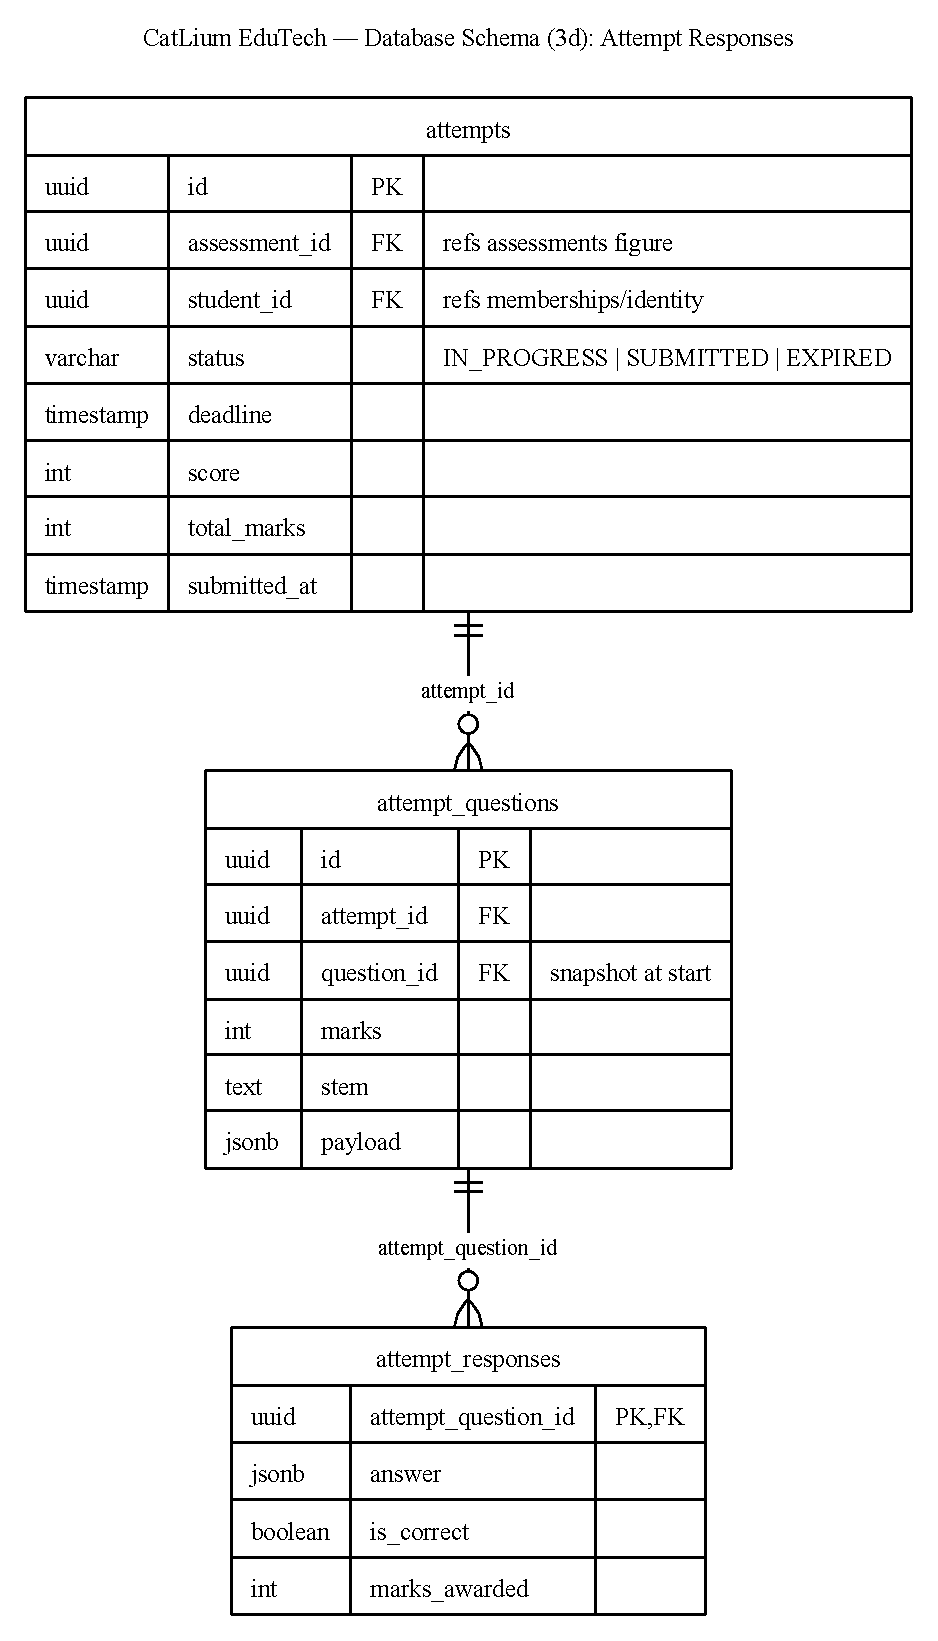
\includegraphics[width=388.3pt]{figures/erd-attempt-responses-bw.pdf}
\caption{Database schema --- attempt snapshots and response tables.}

\end{figure}
\begin{figure}[p]
\centering
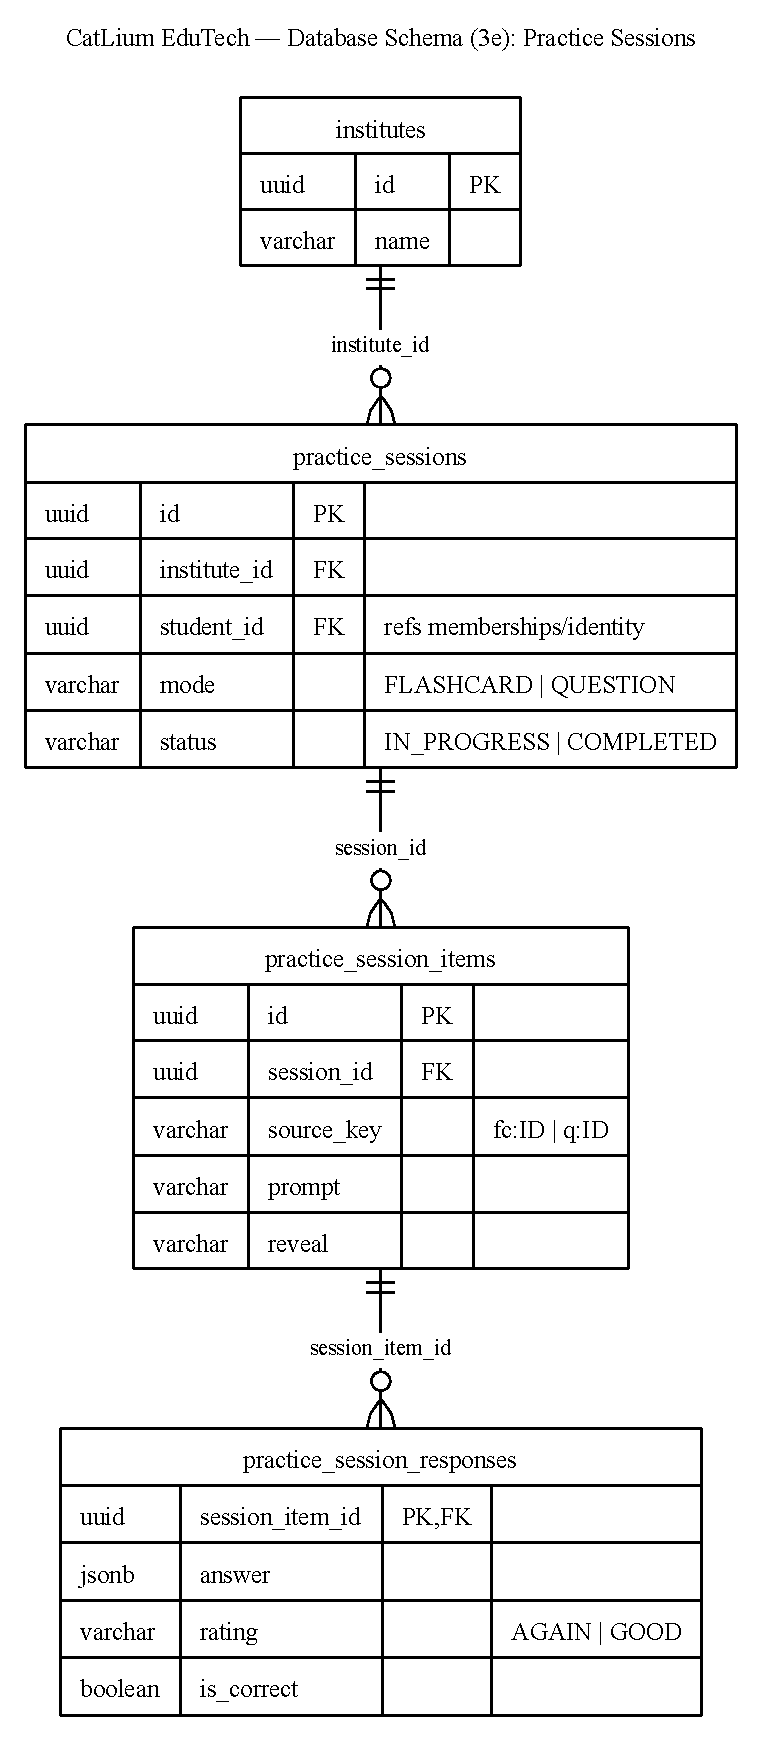
\includegraphics[width=297.7pt]{figures/erd-practice-sessions-bw.pdf}
\caption{Database schema --- ungraded practice sessions.}

\end{figure}
\begin{sidewaysfigure}[p]
\centering
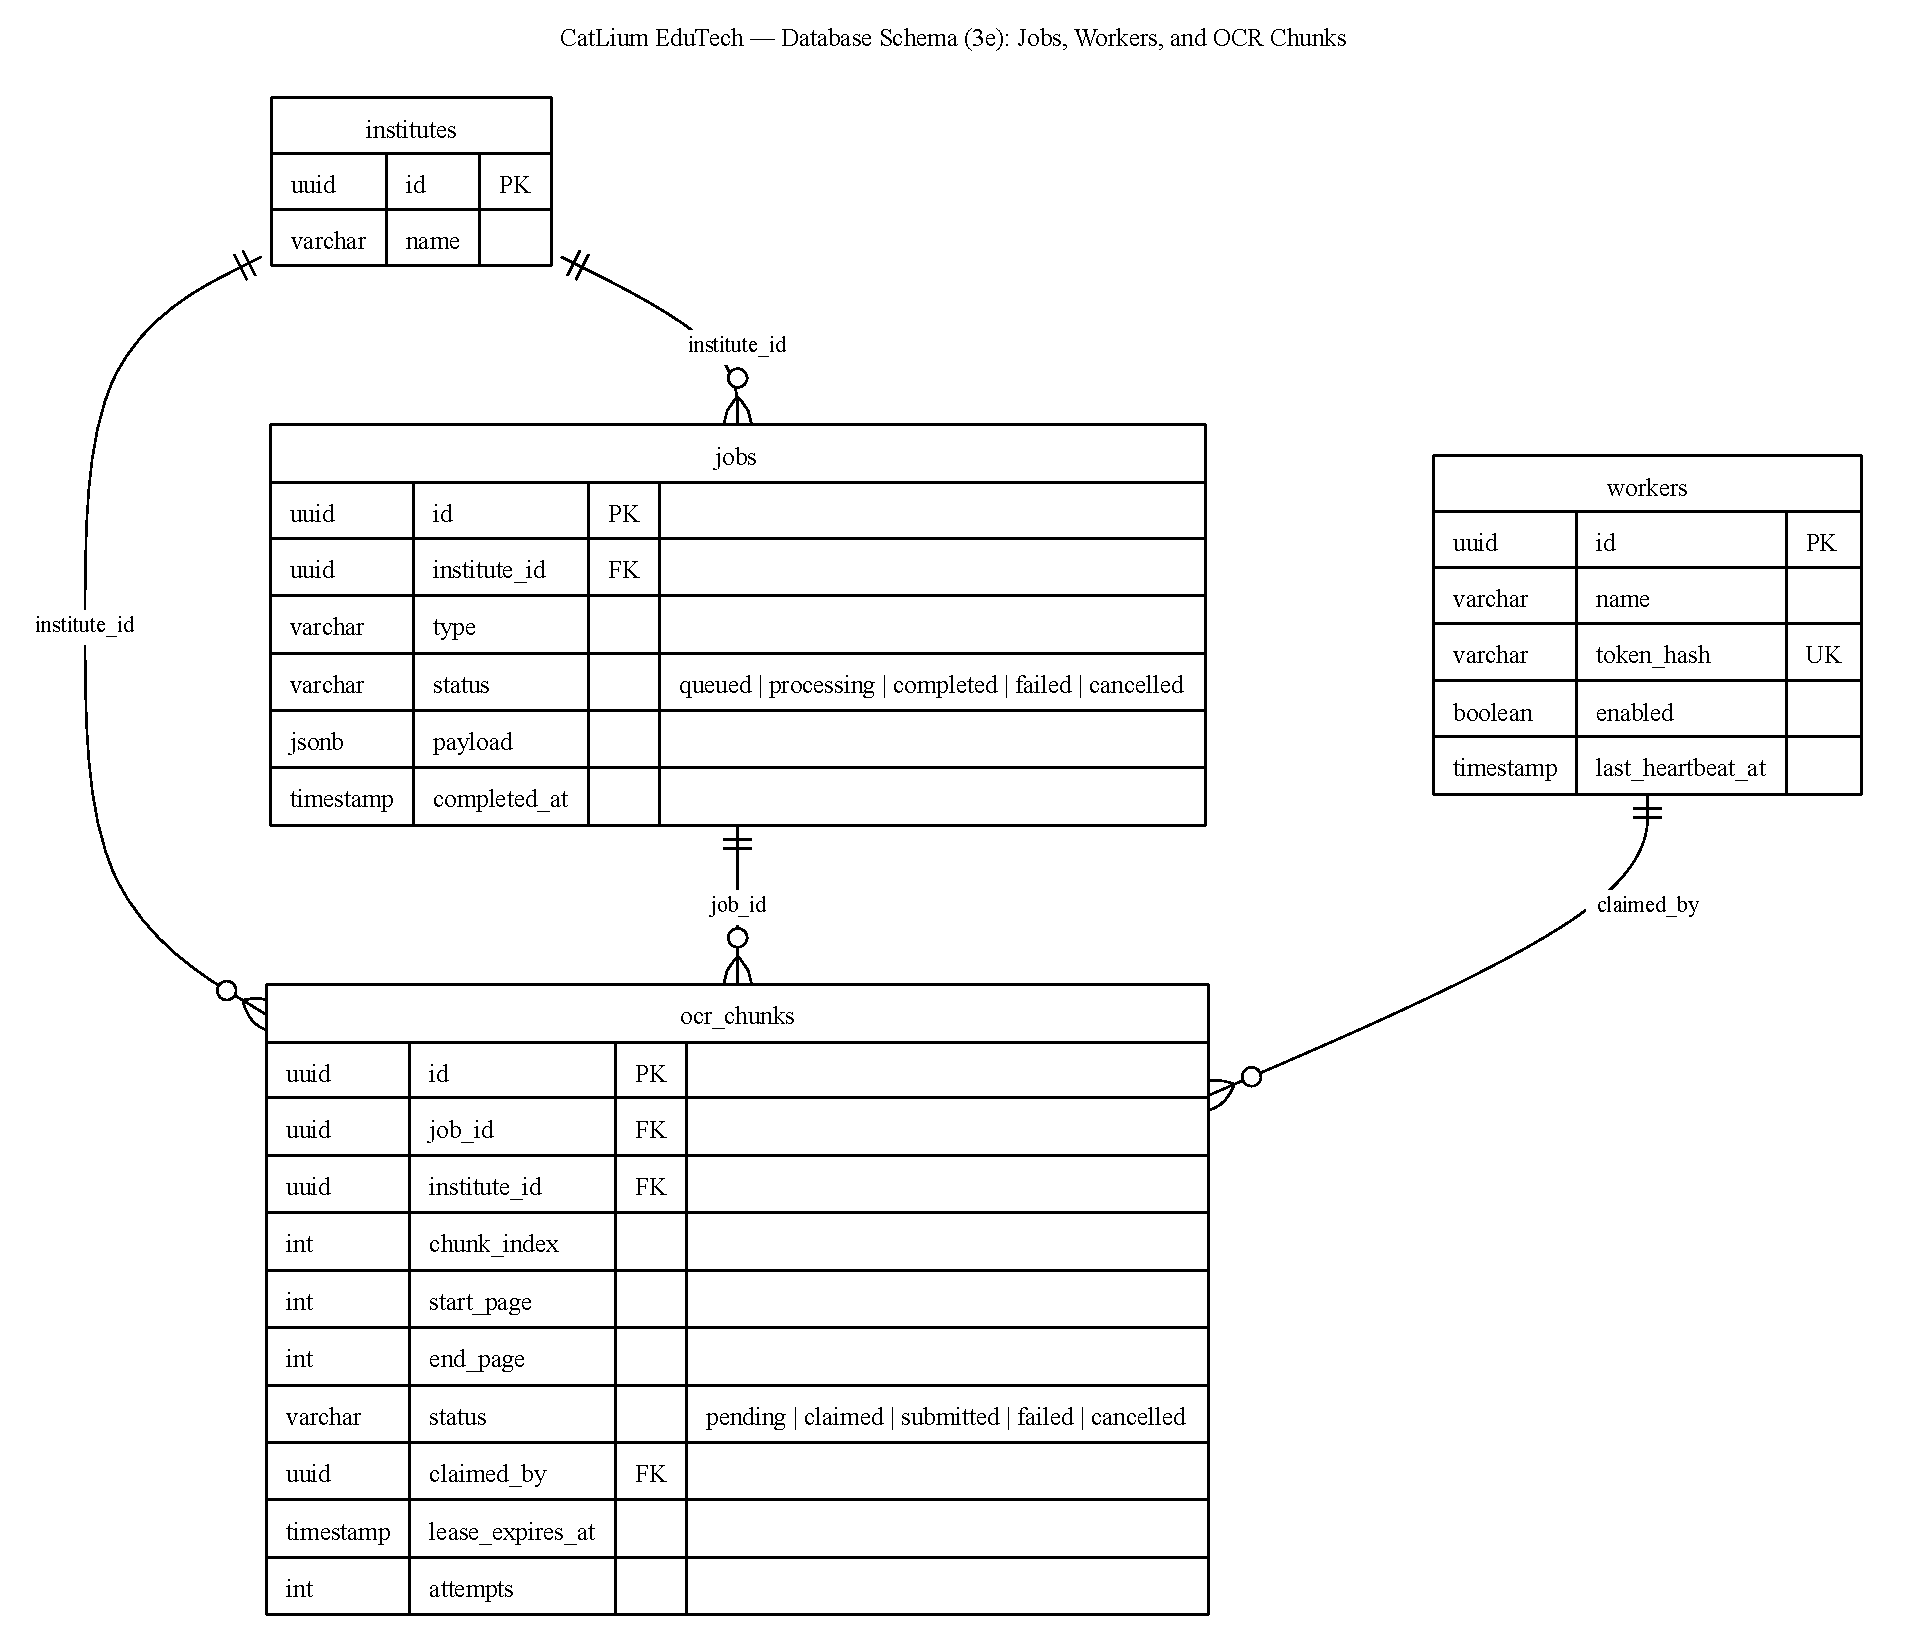
\includegraphics[width=465.6pt]{figures/erd-jobs-ocr-bw.pdf}
\caption{Database schema --- operations: the job/worker/OCR-chunk registry.}

\end{sidewaysfigure}
\begin{sidewaysfigure}[p]
\centering
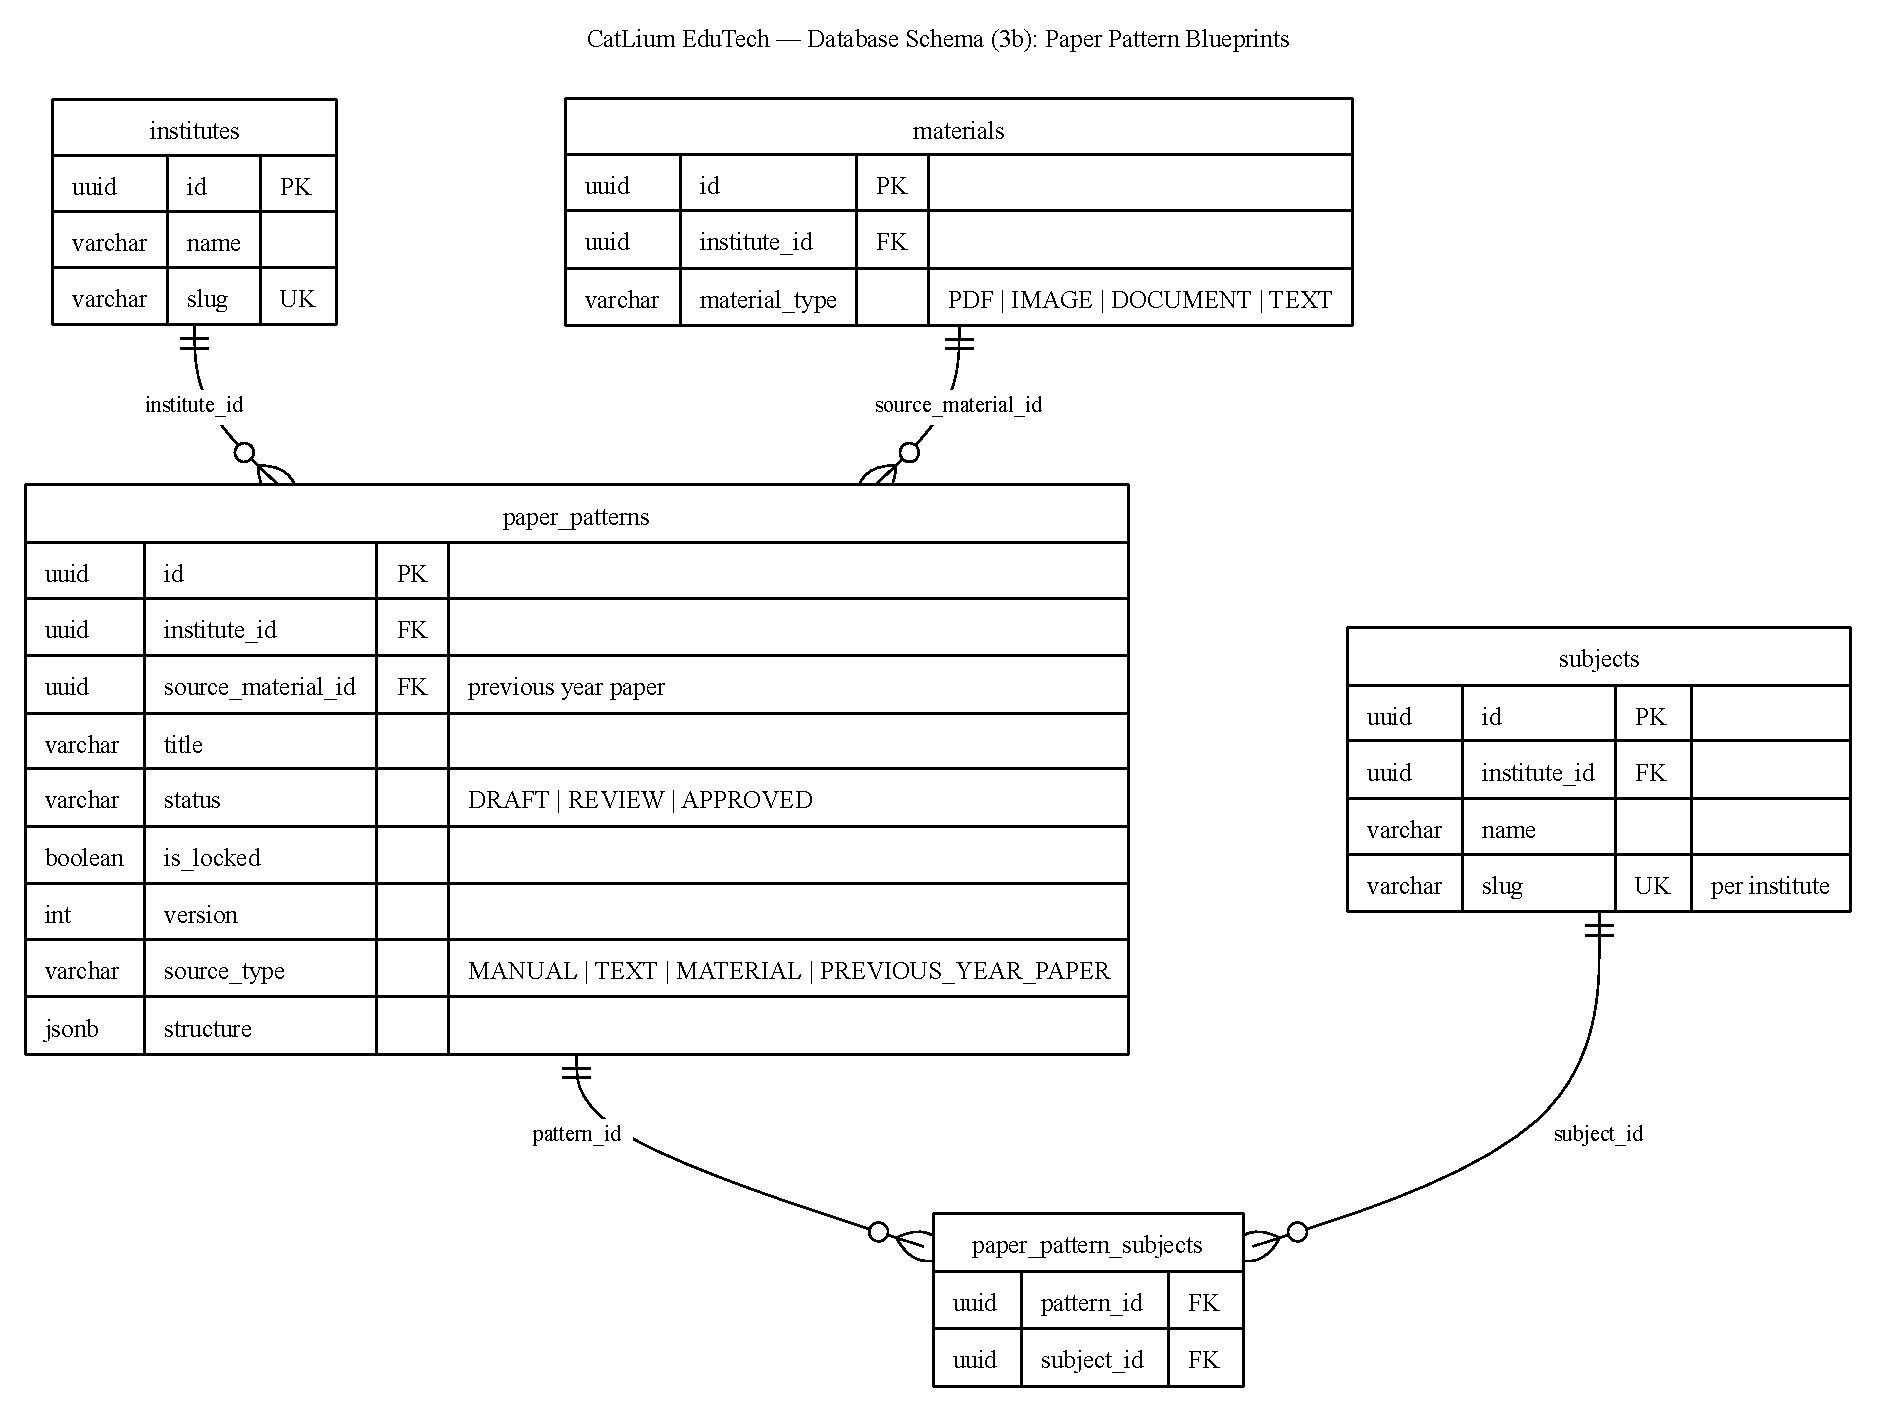
\includegraphics[width=532.2pt]{figures/erd-paper-patterns-bw.pdf}
\caption{Database schema --- operations: paper-pattern blueprints.}

\end{sidewaysfigure}

\chapter{Security and Authorization Architecture}

\begin{sidewaysfigure}[p]
\centering
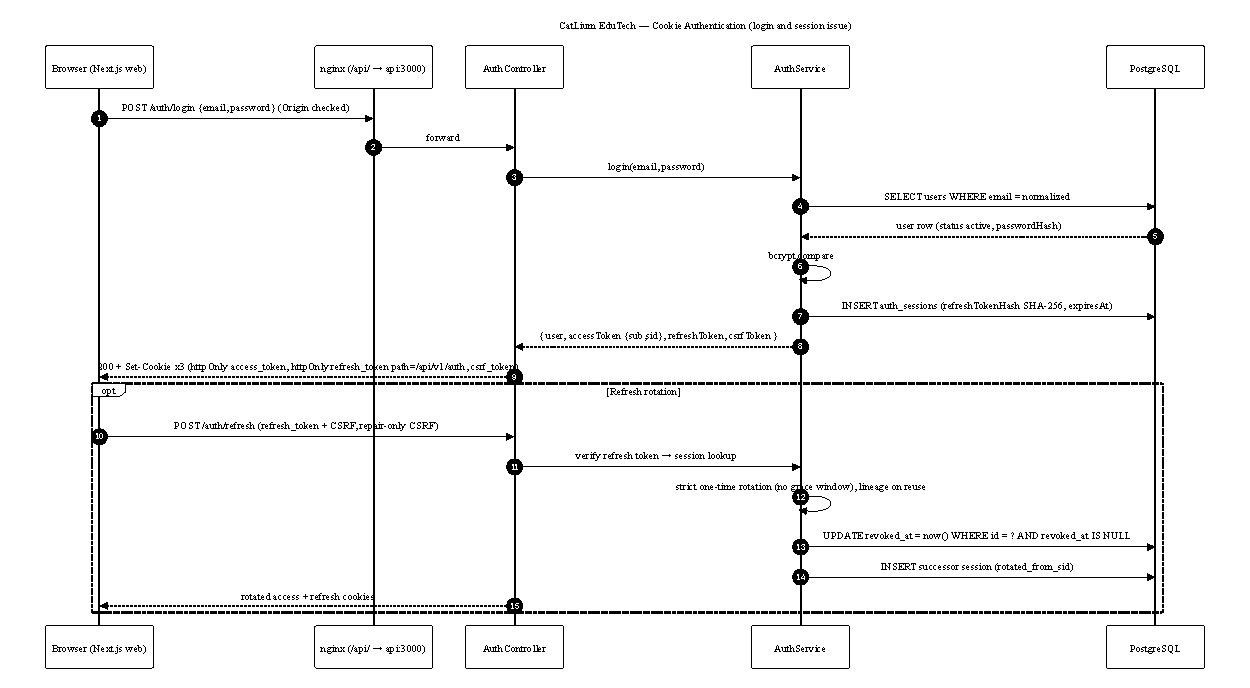
\includegraphics[width=711.5pt]{figures/authentication-login-sequence-bw.pdf}
\caption{Cookie authentication: login, cookie issue, and strict one-time
refresh rotation.}

\end{sidewaysfigure}
\begin{sidewaysfigure}[p]
\centering
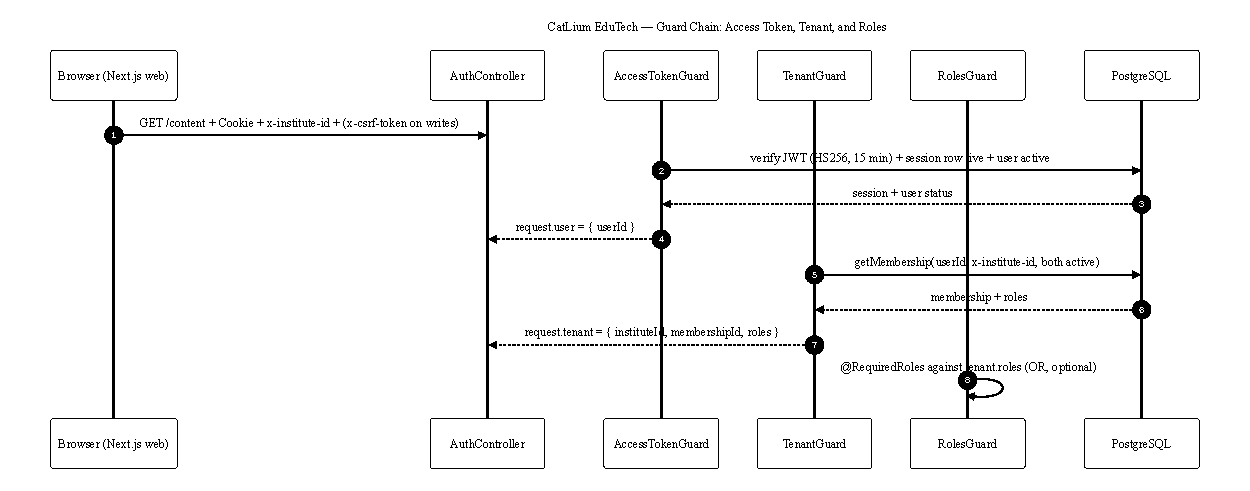
\includegraphics[width=711.5pt]{figures/authentication-guardchain-sequence-bw.pdf}
\caption{Tenant-scoped request flow, part 1: the access-token, tenant, and
roles guards.}

\end{sidewaysfigure}
\begin{sidewaysfigure}[p]
\centering
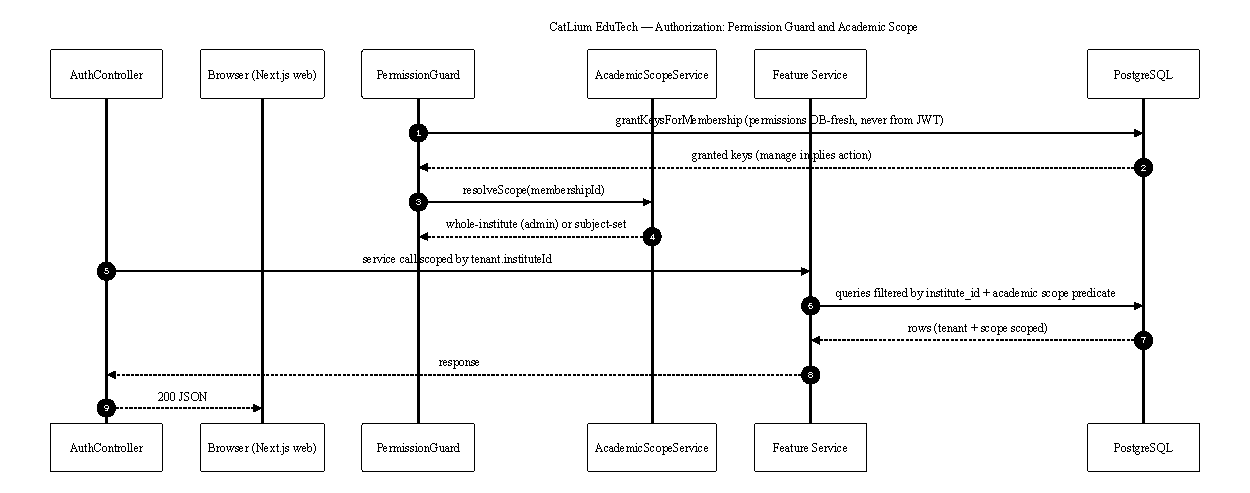
\includegraphics[width=711.5pt]{figures/authentication-authorization-sequence-bw.pdf}
\caption{Tenant-scoped request flow, part 2: permission-guard evaluation and
academic-scope enforcement in the feature service.}

\end{sidewaysfigure}
\begin{figure}[p]
\centering
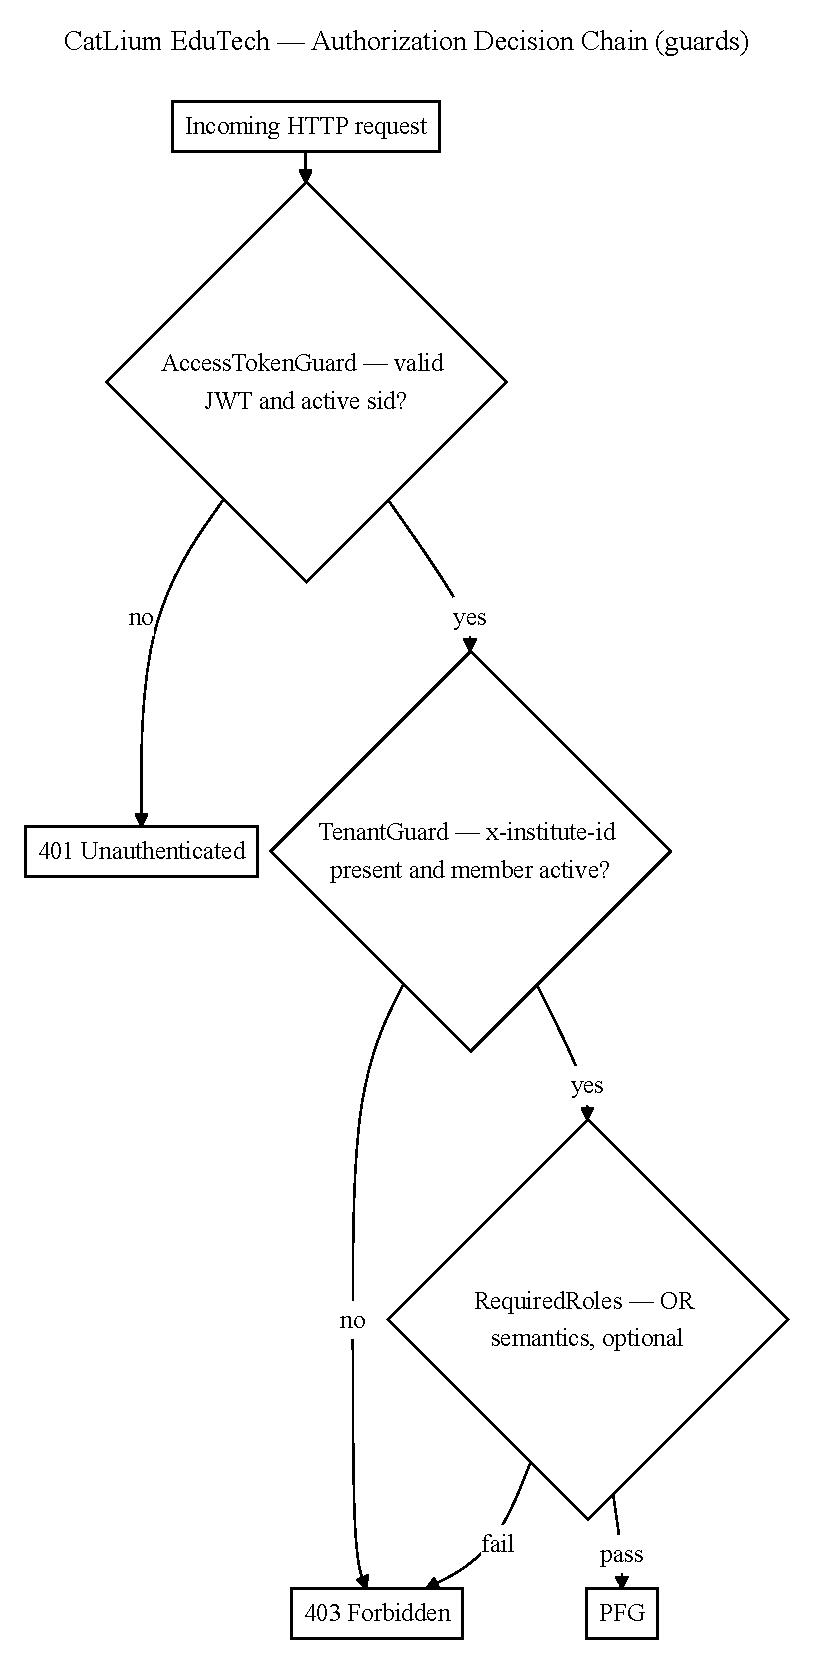
\includegraphics[width=327pt]{figures/permission-model-guards-bw.pdf}
\caption{Authorization decision chain for a tenant-scoped request, part 1:
the guard-stage decisions.}

\end{figure}
\begin{figure}[p]
\centering
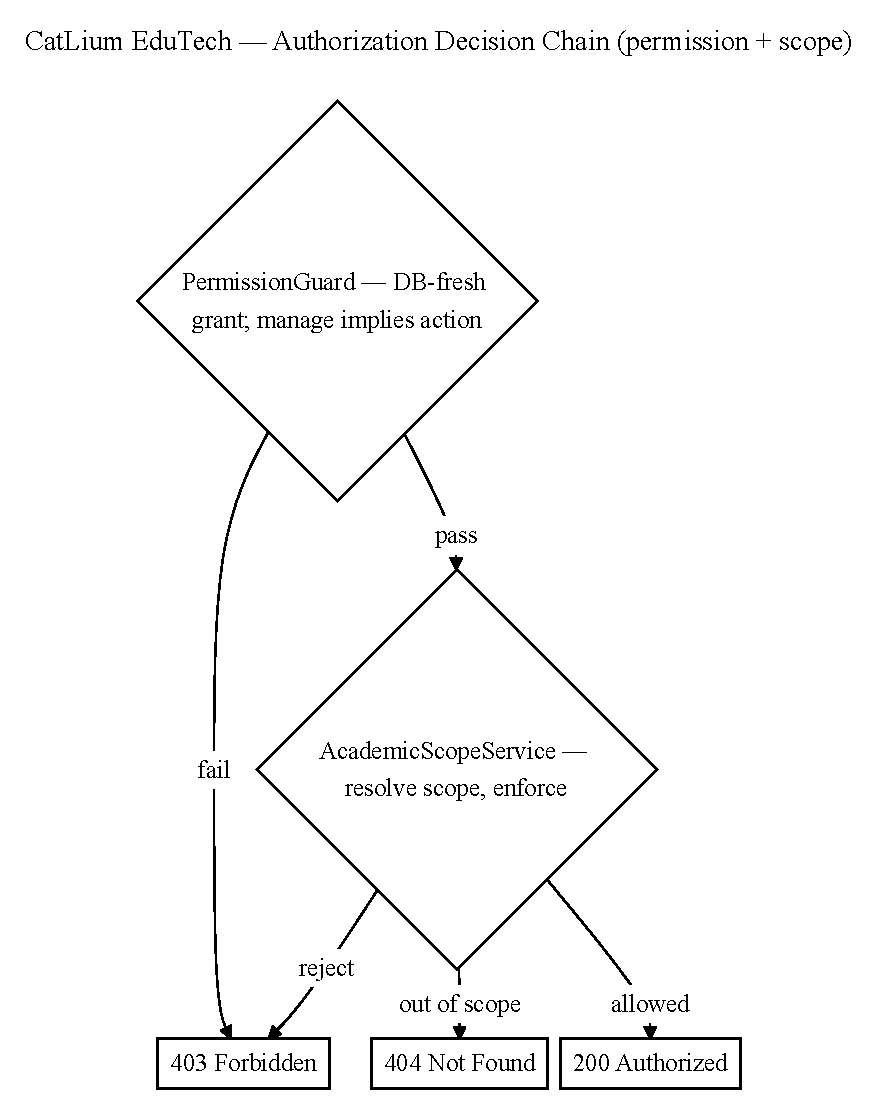
\includegraphics[width=436.5pt]{figures/permission-model-scope-bw.pdf}
\caption{Authorization decision chain for a tenant-scoped request, part 2:
permission evaluation and academic-scope enforcement outcomes.}

\end{figure}
\begin{figure}[p]
\centering
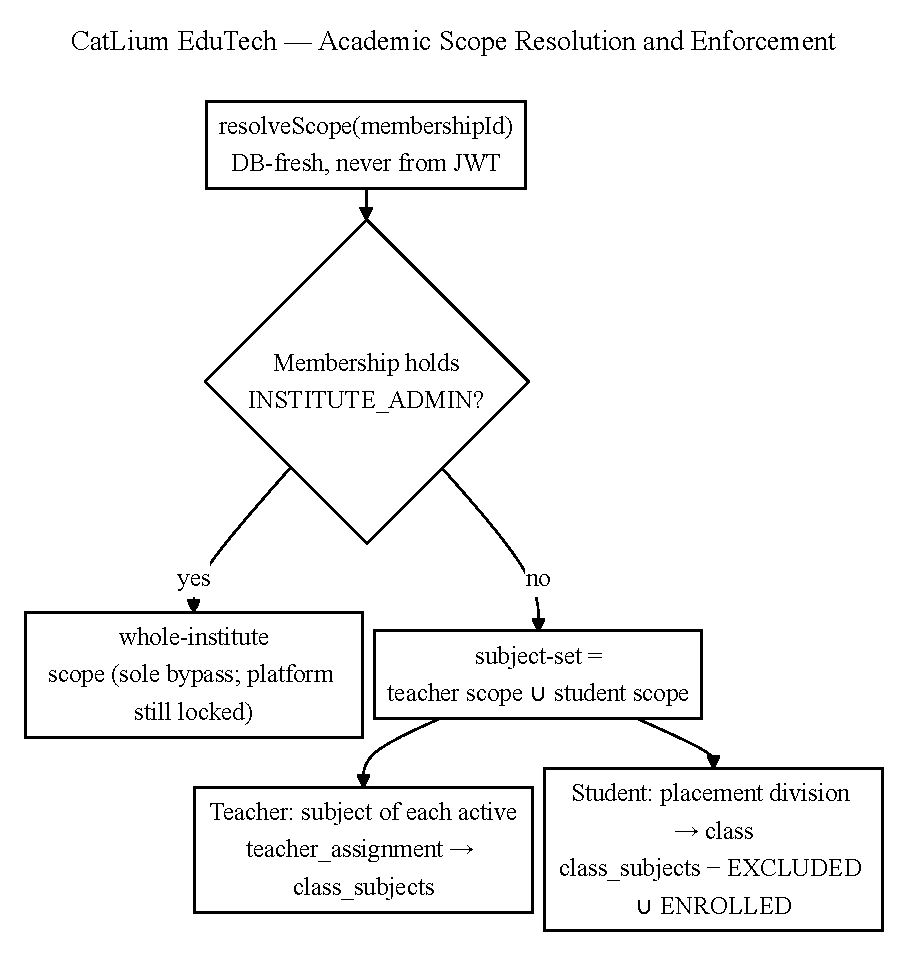
\includegraphics[width=436.5pt]{figures/academic-scope-resolution-bw.pdf}
\caption{Academic scope --- resolution of the actor's subject set from
database state.}

\end{figure}
\begin{sidewaysfigure}[p]
\centering
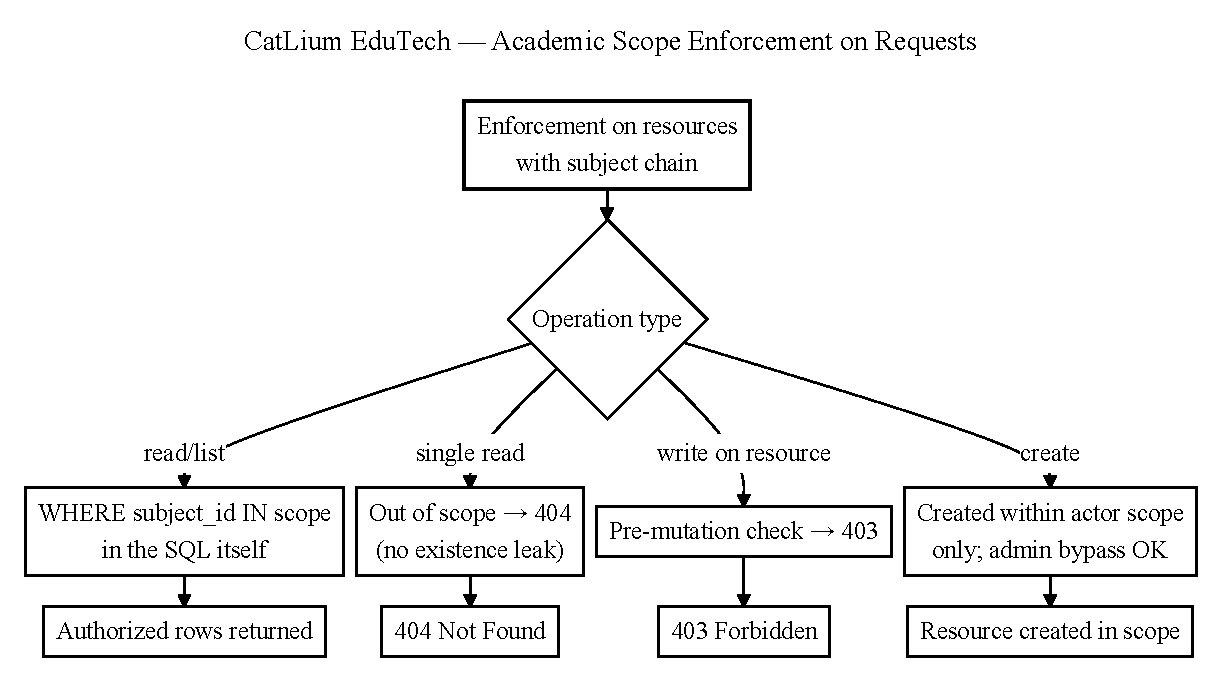
\includegraphics[width=711.5pt]{figures/academic-scope-enforcement-bw.pdf}
\caption{Academic scope --- enforcement outcomes (reads 404, writes 403).}

\end{sidewaysfigure}

\chapter{Core Features and Workflows}

\begin{sidewaysfigure}[p]
\centering
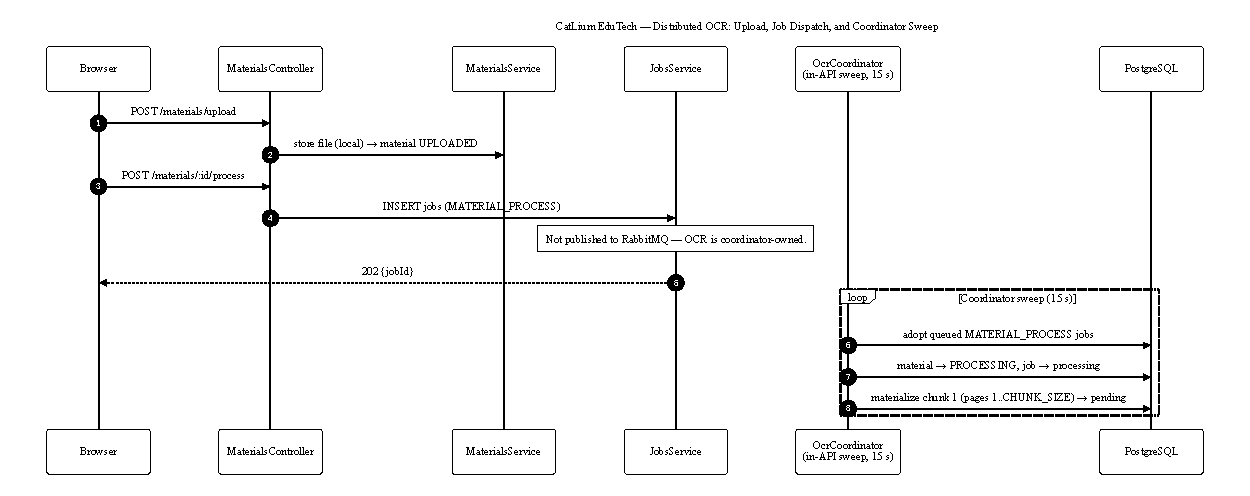
\includegraphics[width=711.5pt]{figures/ocr-flow-coordinator-sequence-bw.pdf}
\caption{Distributed OCR material processing, part 1: upload, job dispatch,
and the coordinator sweep.}

\end{sidewaysfigure}
\begin{figure}[p]
\centering
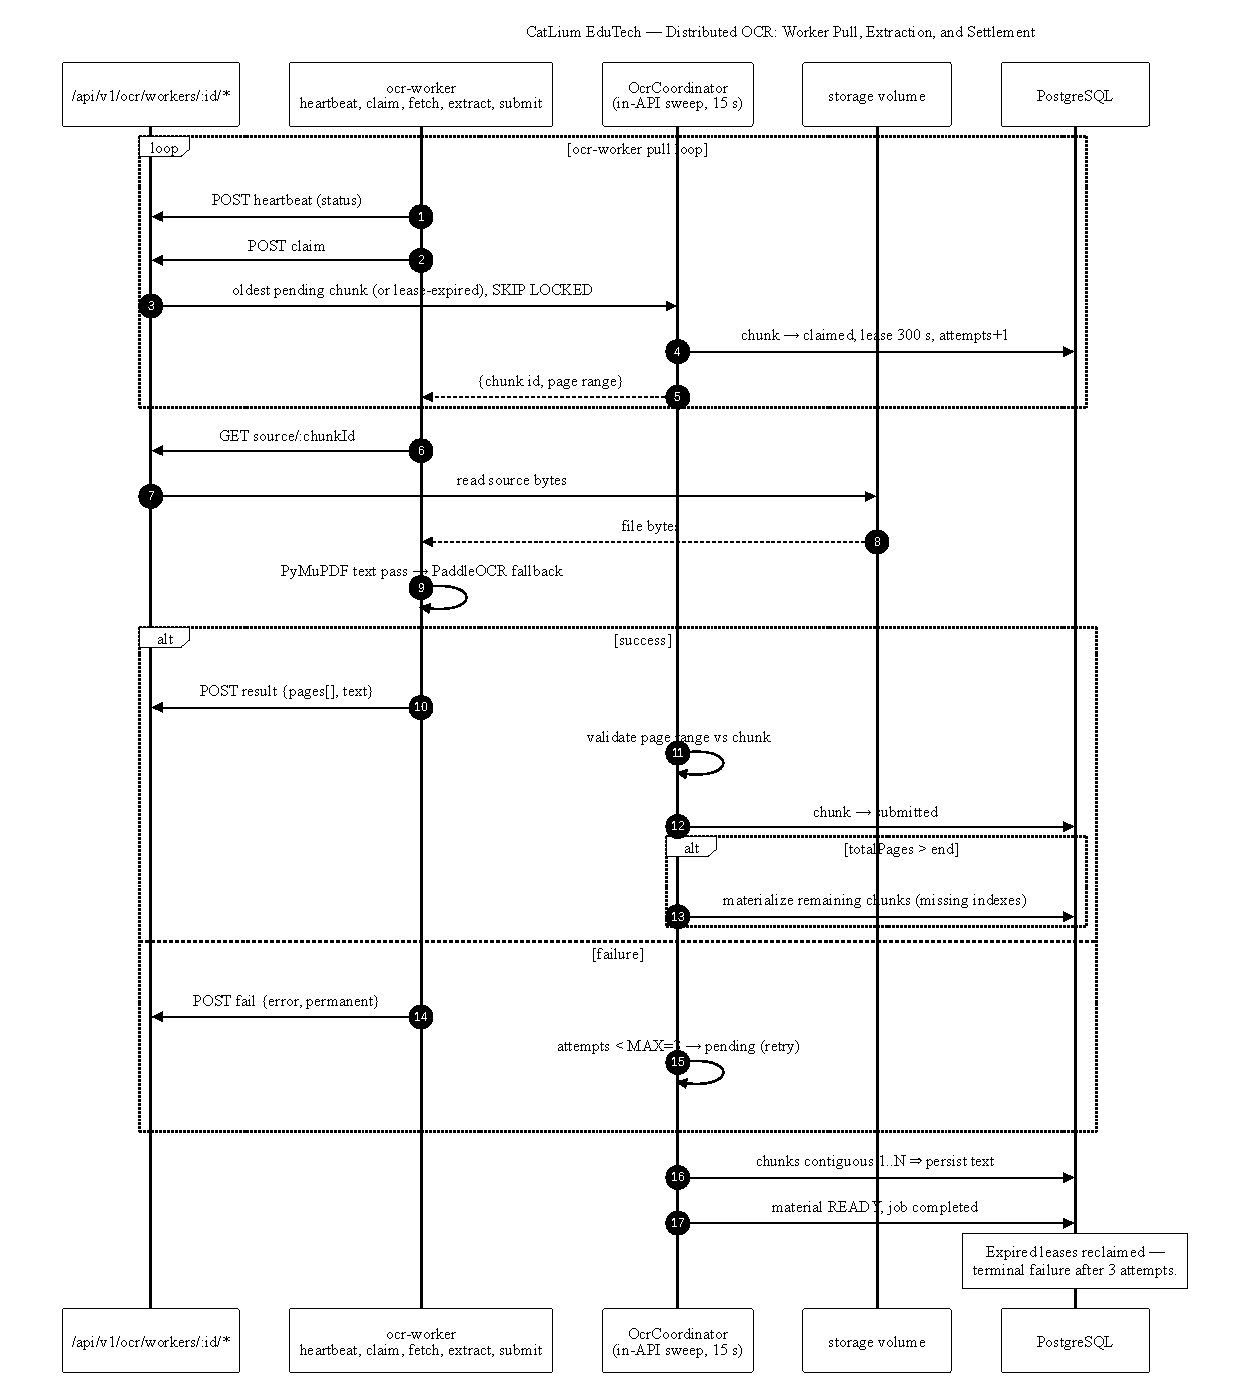
\includegraphics[width=436.5pt]{figures/ocr-flow-worker-sequence-bw.pdf}
\caption{Distributed OCR material processing, part 2: worker pull, extraction,
and settlement.}

\end{figure}
\begin{sidewaysfigure}[p]
\centering
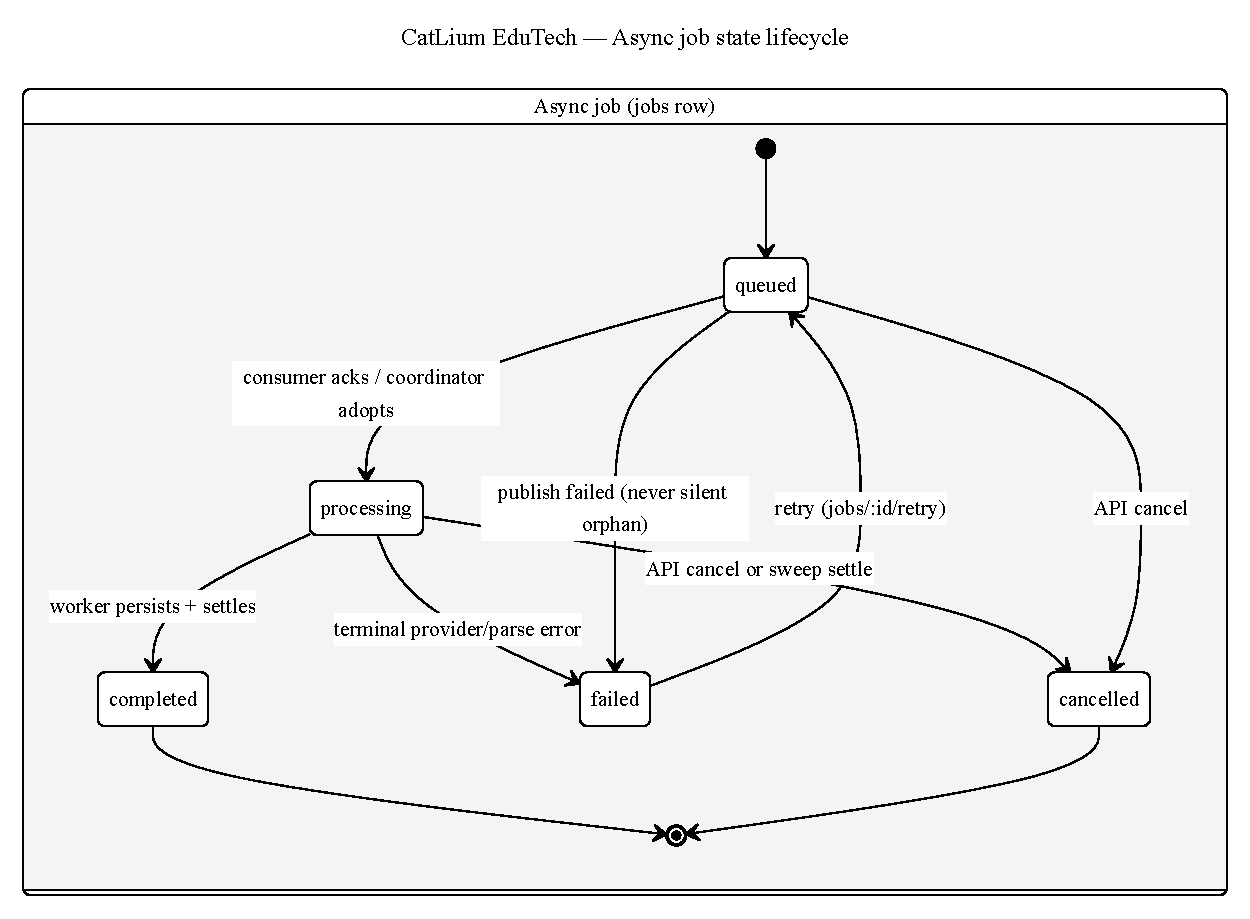
\includegraphics[width=544.9pt]{figures/state-job-lifecycle-bw.pdf}
\caption{Job state lifecycle.}

\end{sidewaysfigure}
\begin{sidewaysfigure}[p]
\centering
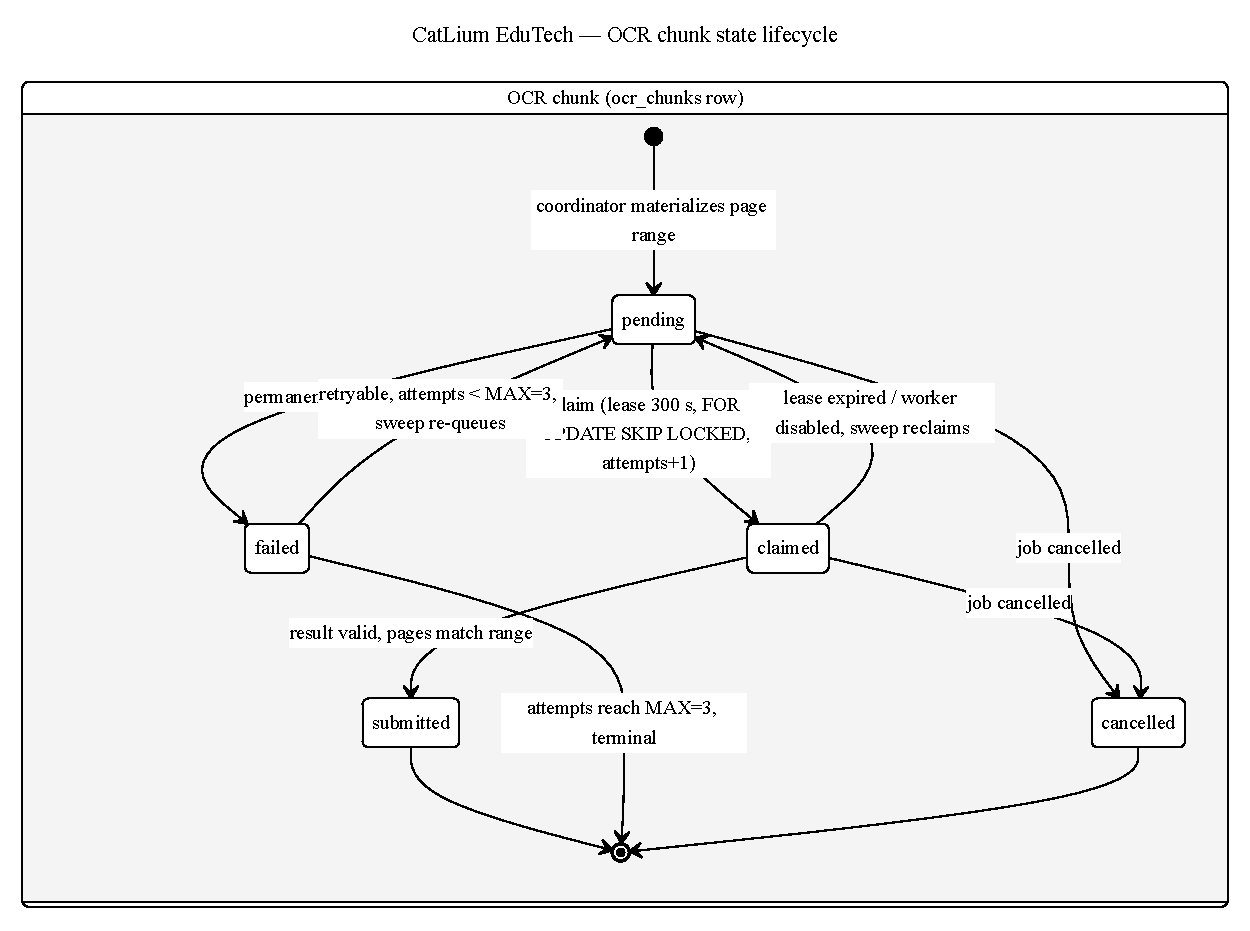
\includegraphics[width=537.6pt]{figures/state-chunk-lifecycle-bw.pdf}
\caption{OCR chunk state lifecycle.}

\end{sidewaysfigure}
\begin{sidewaysfigure}[p]
\centering
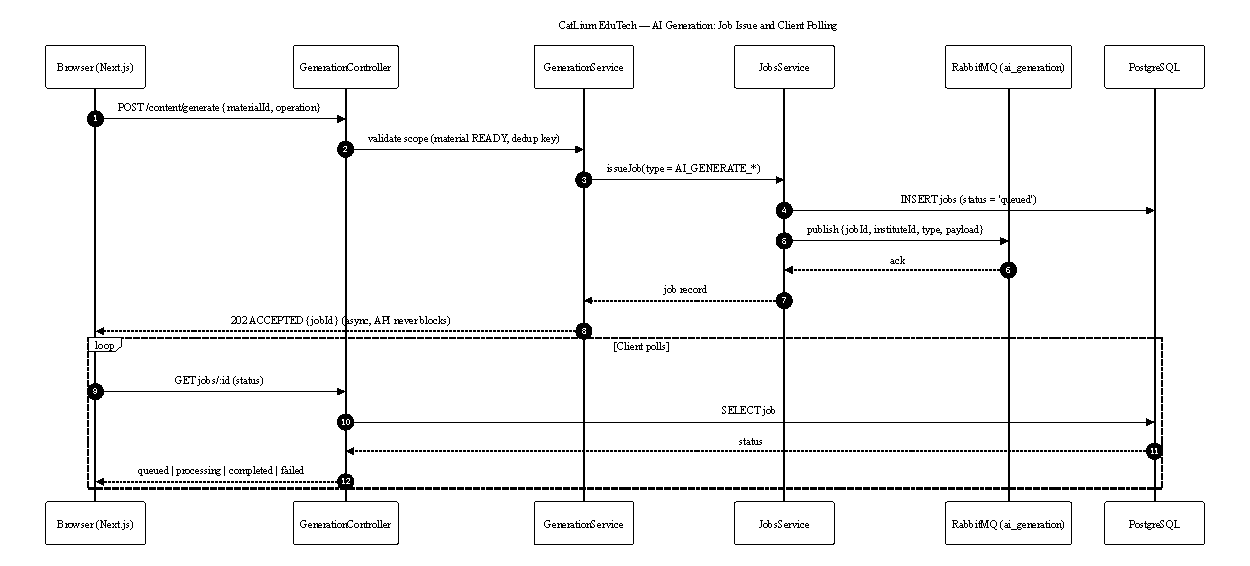
\includegraphics[width=711.5pt]{figures/ai-generation-issue-sequence-bw.pdf}
\caption{Asynchronous AI generation, part 1: job issue and client polling.}

\end{sidewaysfigure}
\begin{sidewaysfigure}[p]
\centering
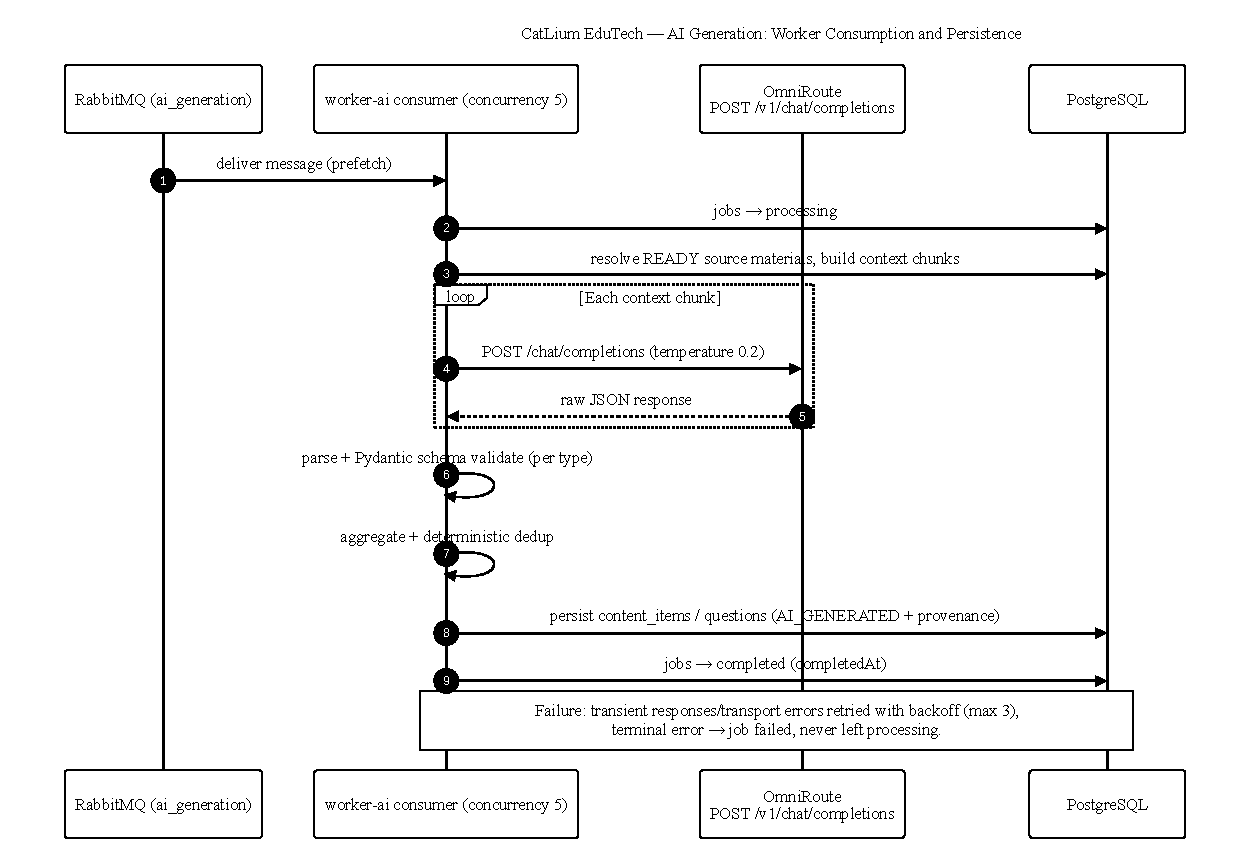
\includegraphics[width=580.4pt]{figures/ai-generation-consume-sequence-bw.pdf}
\caption{Asynchronous AI generation, part 2: worker consumption, OmniRoute
calls, and persistence.}

\end{sidewaysfigure}
\end{document}
